\chapter{Fundamentals}
\label{chap:fundamentals}
This chapter introduces the terminology employed throughout this work, followed by a brief overview of \acf{ML} fundamentals, including supervised, unsupervised, and reinforcement learning. The focus then shifts to semantic segmentation, exploring its connection to \acf{CV}, segmentation objectives, metrics, and architectures.
\section{Terminology}
\label{sec:terminology}
This section provides the terminology used throughout this work to guarantee consistency for mathematical definitions. The terms are commonly used within \ac{ML} and have been adapted to fit the context of semantic segmentation.

\textbf{Input features $x\in X$}: Data from the input space $X$ which we want to use to make predictions for. In the case of semantic segmentation, every input $x$ can be defined as a tensor of shape $([C,H,W])$ where $C$ is the number of channels such as red-green-blue (RGB), $H$ the height and $W$ the width of the image. If we use batches of images, we describe them as a tensor of $([N,C,H,W])$ where $N$ is the number of batches.

\textbf{Output labels $y\in Y$}: Targets from the label space which we want to predict. Labels consist of tensors of shape $([N,H,W])$ where $N$ is the batch size, $H$ is the height, and $W$ is the image's width. For training, we usually convert the tensor $([N,H,W])$ into a one-hot-encoded format of shape $([N,D,H,W])$ where $D$ stands for the number of distinct classes.

\begin{figure}[H]%[htbp]
    \centering
    \subfigure[]{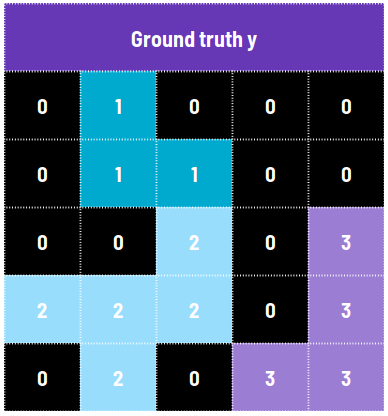
\includegraphics[width=\imgWidthFive]{images/oneHotEncoding_1.png}}
    \subfigure[]{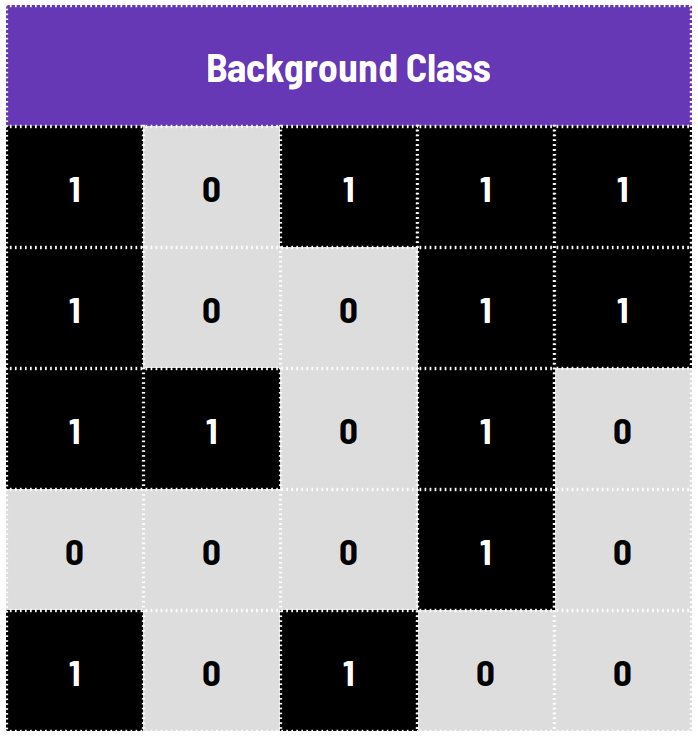
\includegraphics[width=\imgWidthFive]{images/oneHotEncoding_5.png}}
    \subfigure[]{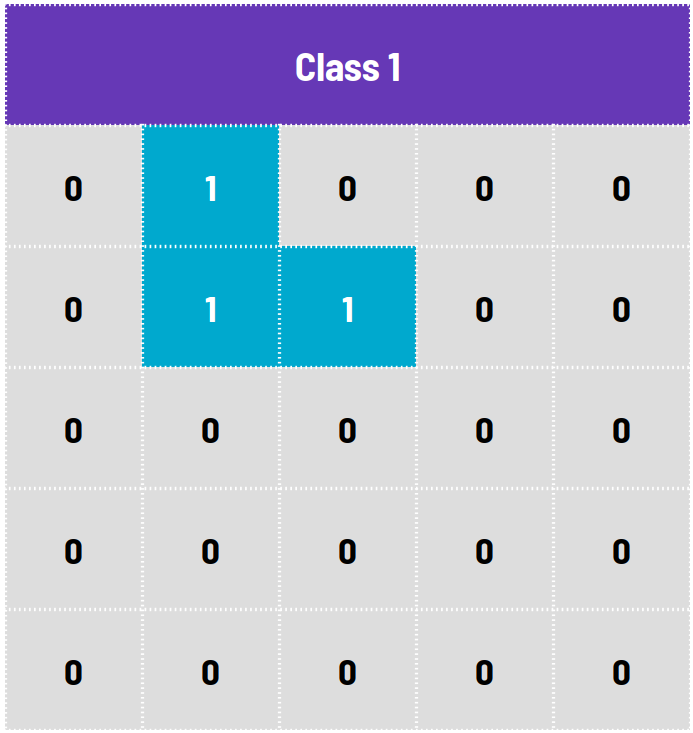
\includegraphics[width=\imgWidthFive]{images/oneHotEncoding_2.png}}
    \subfigure[]{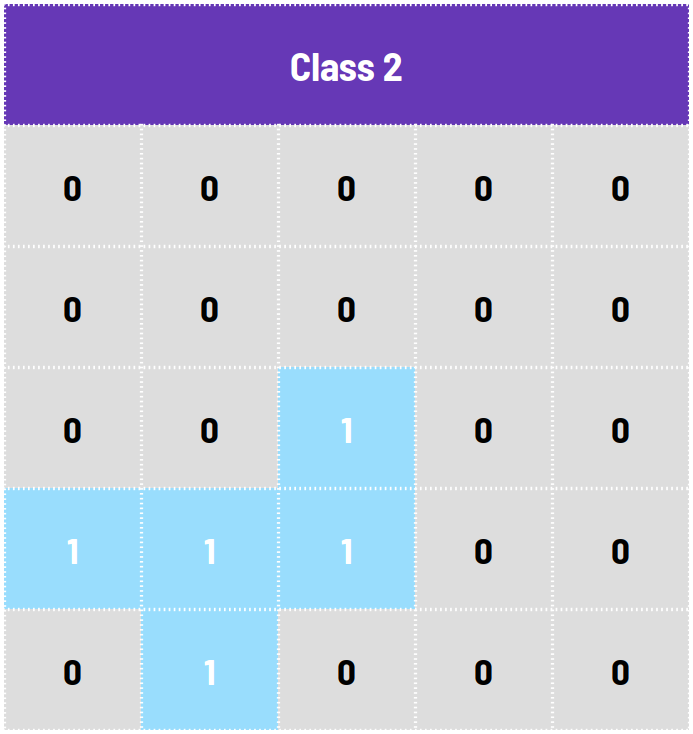
\includegraphics[width=\imgWidthFive]{images/oneHotEncoding_3.png}}
    \subfigure[]{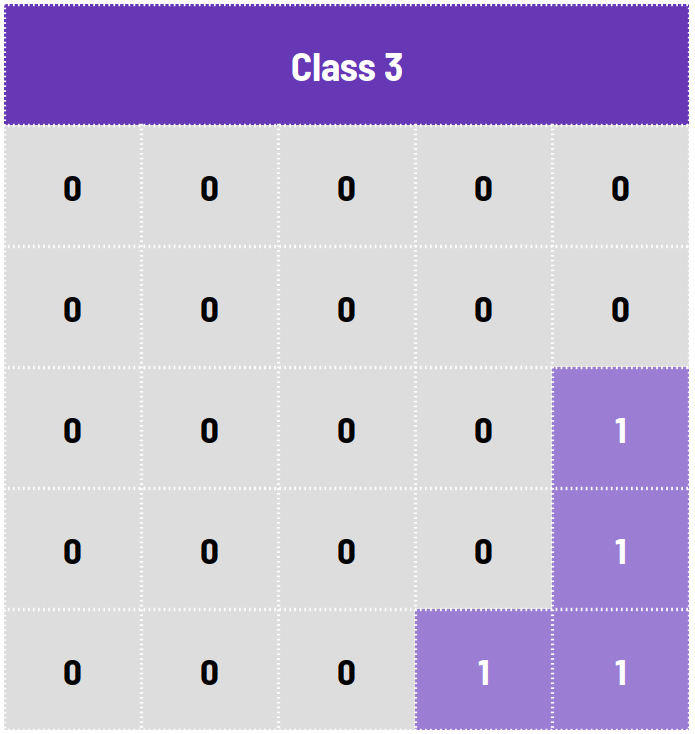
\includegraphics[width=\imgWidthFive]{images/oneHotEncoding_4.png}}
    \caption[Integer encoding $\to$ one-hot-encoding]{Example of integer-encoded output label (a) transferred to a one-hot-encoded label (b-e) of shape $([N,D,H,W])$. In this example, the batch size $N=1$}
    \label{one_hot_encoded_mask}
\end{figure}

\textbf{Probability distribution $\mathbb{P}(XY)$}: Unknown distribution of input features and output labels. A subset from this distribution would be a dataset $D=\{(x_i,y_i)\}_{i=1}^m \in (X,Y) \sim \mathbb{P}(X,Y)$.

\begin{figure}[H]%[htbp]
    \centering
    \subfigure[]{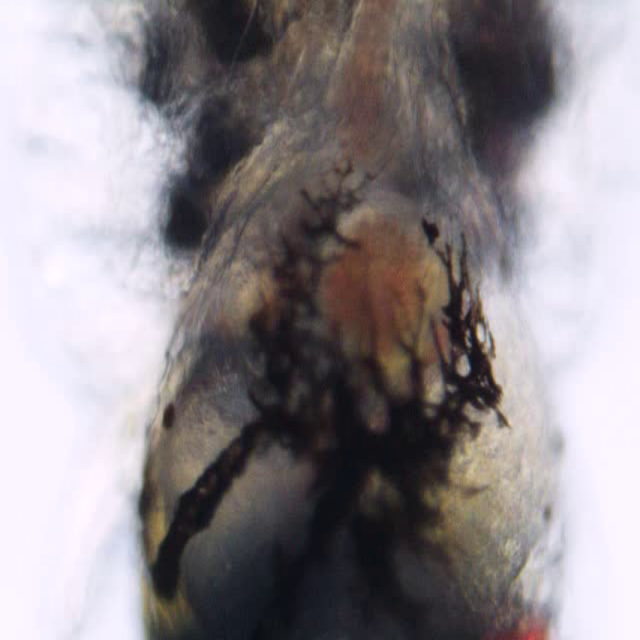
\includegraphics[width=\imgWidthTwo]{images/medaka.png}}
    \subfigure[]{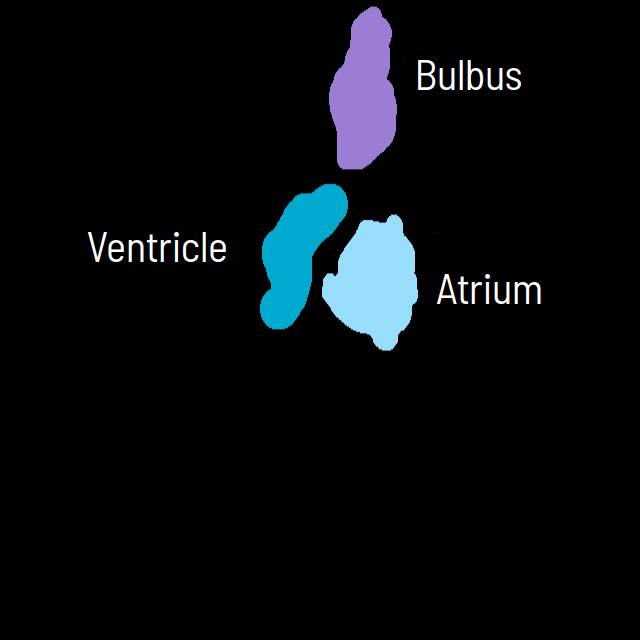
\includegraphics[width=\imgWidthTwo]{images/00020_mask.png}}
    \caption[Sample label pair]{Example of sample (a) label (b) pair $(x_1,y_1)\in (X,Y)$ of the Medaka fish dataset with four classes (Bulbus, Ventricle, Atrium, and Background)}
    \label{sample_label_pair}
\end{figure}

\textbf{Model $h_{\theta}:X \to \hat{Y}$}: Function to map features from the input space $X$ to the prediction space $\hat{Y}$ depending on $\theta$. Within semantic segmentation, $h_{\theta}$ consists of a \acf{CNN}.

\textbf{Parameters $\theta \in \Theta$}: Weights of the model which are intended to be optimized during the training phase of the model.

\textbf{Predictions $\hat{y}\in \hat{Y}$}: Outputs of the model $h_{\theta}$. The value typically consists of scores inferred from the model $h_{\theta}$. For segmentation tasks, the output shape $\hat{Y}$ is usually of the form $([N,D,H,W])$ such as $Y$, and is then optionally transformed into probabilities as defined in \secref{sec:softmax}.

\textbf{Loss function $l:\hat{Y}\times Y \to \mathbb{R}_+$}: Also known as cost function measures the difference between the prediction $\hat{Y}$ and the output label $Y$. The goal of a machine learning model is to minimize the value of the loss function by providing a gradient or direction for the model to make.


\section{Machine Learning}
\acf{ML} is a subfield of \acf{AI}. The paper \squote{Machine learning: Trends, perspectives, and prospects}\cite{doi:10.1126/science.aaa8415} provides an excellent summary of \ac{ML} and defines it as the question of \squote{How to build computers that improve automatically through experience}. The paper starts by outlining its importance as one of today's most rapidly growing technical fields and as a method of choice in \acf{CV}, \acf{NLP}, \acf{SR}, or \acf{RC}. It formally defines \ac{ML} as a learning problem to improve some measure of performance when executing some task through some training experience. Further, it describes the three most important paradigms of \ac{ML} known as \acf{SL}, \acf{UL}, and \acf{RL}.

\subsection{Supervised Learning}
\label{subsec:supervised_learning}
\acf{SL} techniques are nowadays the most widely used methods \cite{doi:10.1126/science.aaa8415}. Those methods are based on the principle known as \ac{ERM} from statistical learning theory \cite{NIPS1991_ff4d5fbb}. It is defined as an approach of the \squote{expected risk} as
\begin{equation}
    R(h_\theta)=\mathbb{E}[L(h(X),Y)]=\int L(h(X),Y) d\mathbb{P}(X,Y)
    \label{eqn:expected_risk}
\end{equation}
with the \squote{empirical risk} as
\begin{equation}
    R_\delta(h_\theta)=\int l(h_\theta(X),Y)d \mathbb{P}_\delta(X,Y)=\frac{1}{m}\sum_{i=1}^m l(h_\theta(x_i),y_i)
    \label{eqn:empirical_risk}
\end{equation}
The idea is that even if we do not know the real joint distribution of a sample, label pairs $\mathbb{P}(X,Y)$, we still can approach it with some known training data. The general goal of a \ac{SL} algorithm is to find a function $h \in H$ which models the relationship between a random feature vector $X$ and a random target vector $Y$, also called output label, by following the joint distribution $\mathbb{P}(X,Y)$. $L$ is the loss function which penalizes the differences between prediction $h(x)$ and $Y$. $\mathbb{E}[L(h(x),y)]$ is the expected loss if we obtain samples from the same distribution $\mathbb{P}(x,y)$ as the training data \cite{DBLP:journals/corr/abs-1710-09412}. The difference between \ref{eqn:expected_risk} and \ref{eqn:empirical_risk} is the distribution from where the data is sampled. While the former samples the data from the real unknown distribution $\mathbb{P}(X,Y)$, the latter is an approximation obtained from the distribution $\mathbb{P}_\delta(X,Y)$ wich represents samples from a dataset $DS=\{(x_i,y_i)\}_{i=1}^m$.

The inputs of the dataset $DS$ can have numerous forms, such as simple vectors, DNA sequences, images, or graphs \cite{doi:10.1126/science.aaa8415}. For \ac{SL} methods, the output $y$ typically is either a category used for classification or a real value for regression methods. The following section will describe some of the most essential \ac{SL} methods and briefly outline how to optimize the \squote{empirical risk} defined as \ref{eqn:empirical_risk}.

\subsubsection*{Supervised Learning Models}
\label{subsubsec:supervised_learning_models}
\textbf{\emph{\acf{LR}}} is a supervised technique used to model the relationship between a dependent and one or more independent variables. The dependent variable is a real value. Some applications for \ac{LR} are the prediction of stock prices for financial institutes \cite{bhuriya2017stock}, sales volume \cite{todua2013multiple}, customer lifetime value \cite{malthouse2005can} or churn rates \cite{hadden2008churn} for sales and marketing departments \cite{maulud2020review}, predicting patient outcomes \cite{lewis2007regression} or healthcare costs \cite{soyiri2013overview}, modeling the relationship between environmental variables such as temperature \cite{radhika2009atmospheric}, humidity \cite{vamseekrishna2021prediction} or precipitation \cite{naoum2004orographic} and their impact on natural systems for environmental scientists \cite{shen2015precipitation}. Mathematically, the linear regression model can be expressed as
\begin{equation}
    h_{\theta}(x)= \sum_{j=1}^n \theta_j x_j=\theta^T x
    \label{eqn:linear_regression}
\end{equation}
where $x$ is the dependent variable, $h_\theta(x)$ the independent variables and $n$ the number of features. $\theta$ are the coefficients or parameters. As a loss function, we could use the squared error or $l_1$ loss defined as
\begin{equation}
    l_1(h_{\theta}(x),y)=\sum_{i=1}^m(\theta^T x_i-y)^2
\end{equation}
or the absolute loss or $l_2$ as
\begin{equation}
    l_2(h_{\theta}(x),y)=\sum_{i=1}^m|\theta^T x_i-y|
\end{equation}
which is less sensitive to outliers \cite{thanoon2015robust}\cite{su2012linear}. Note that $m$ is the number of samples in the dataset.

\textbf{\emph{\acf{LogR}}} is another supervised technique but used for classification problems. The dependent variable is based on a logistic model, which typically estimates the probability of an outcome of two classes. There are many domains where \ac{LogR} can be applied. Some of them are fraud detection \cite{sahin2011detecting}, customer churn prediction \cite{de2018new}, medical diagnosis \cite{tsien1998using} or sentiment analysis \cite{ramadhan2017sentiment}. For \ac{LogR}, we can use the same linear model as defined in \ref{eqn:linear_regression} but with a different loss function as
\begin{equation}
    \begin{split}
        l_{\log}(h_{\theta}(x),y) & =\sum_{i=1}^m y_i \log(\theta^T x_i) + (1-y_i)\log(1-(\theta^T x_i))\\
        & =\sum_{i=1}^m y_i \theta^T x_i - \log(1+ \exp(\theta^T x_i))
    \end{split}
\end{equation}
which is also called the log-likelihood function \cite{hastie2009elements}.

\textbf{\emph{\acf{TBM}}} are also \ac{SL} methods which can be either used for classification or regression tasks. \ac{TBM} can be used with ensemble methods to improve performance. The core idea of ensembles is that, on average, they perform better than individual models. New predictions are then made by averaging \cite{hastie2009elements} or voting \cite{cootes2012robust}. Averaging is used for regression and voting for classification tasks. The advantage of decision trees is that they are easy to create \cite{almuallim2002development} and interpret \cite{kingsford2008decision}, that they require fewer data preparation, and that they are insensitive against outliers or missing data \cite{decisionTreesAdvantages}. Formally the model of \ac{TBM} can be described as
\begin{equation}
    h_\theta(x)=\sum_{m=1}^M c_m \mathbbm{1}\{x \in R_m\}
\end{equation}
The model consists of a sum of constants $c$, if $x$ is within a region $R_m$ of the decision tree. The constants $c_m$ here depend on the task and can be the proportion of each class $c_m=\frac{1}{N_m}\sum_{x_i \in R_m}\mathbbm{1}\{y_i=k\}$ for \acp{CT} or the mean of all labels $c_m=\frac{1}{N_m}\sum_{x_i \in R_m} y_i$ for \ac{RT} \cite{hastie2009elements}. There are numerous popular variants of decision trees such as \ac{RF} \cite{cutler2012random}, \ac{GB} \cite{ke2017lightgbm} or \ac{AB} \cite{wu2020application}.

\textbf{\emph{\acf{KNN}}} is a non-parametric \ac{SL} algorithm. \ac{KNN} can be used for either classification or regression tasks. The predictions for \ac{KNN} are made based on the voting of the majority class among its $k$ nearest neighbors in the training set \cite{doi:10.1142/S0218195905001622}. The advantages of \ac{KNN} are that it is straightforward and easy to understand, that it can achieve high accuracy by using different distance metrics \cite{Uddin2022}, that it can handle non-linear and complex data sets by using kernel functions and that it adapts to changing data distributions by updating nearest neighbors dynamically \cite{zhangzhonghengKNN}. Some disadvantages are that it is slow and computationally expensive for large datasets with many classes \cite{Uddin2022}, its sensitivity to irrelevant features \cite{zhangzhonghengKNN}, and that it suffers from the curse of dimensionality \cite{kouiroukidis2011effects}. Formally the model can be described as
\begin{equation}
    h(x)=\frac{1}{k}\sum_{x_i \in N_k(x)} y_i
\end{equation}
where $N_k(x)$ is the neihborhod of $x$ defined by the $k$ closest points $x_i$ in the data set \cite{hastie2009elements}. This model type can be used for classification where $y=\{-1,+1\}$ or regression where $y$ is a real value.

\textbf{\emph{\acfp{SVM}}} are also \ac{SL} models that can achieve good performance and generalization by using different kernels to handle different types of data and problems. The core idea of \acp{SVM} is to find a linear or non-linear function that maps the input data to a higher-dimensional space where a separating hyperplane with a maximal margin can be found. The hyperplane is defined by a set of points, called support vectors which lie on the boundary of the margin \cite{pisner2020support} \cite{Hearst1998TrendsC}. \acp{SVM} have been extensively used in multiple domains such as text categorization \cite{tong2001support}, face detection \cite{osuna1997training} or neuroimaging analysis \cite{PISNER2020101}. There are numerous types of \acp{SVM}. The soft margin support vector machine in primal form is a minimization of the objective
\begin{equation}
    \begin{split}
        \mathop{\min}_{\theta,b}\quad\quad\frac{1}{2}||\theta||^2 + C \sum_{i=1}^m \xi_i\\
        \text{subject to}\quad y_i(\theta^T f(x_i)+b)&\geq 1 -\xi_i\quad i=1,\hdots ,m\\
        \xi_i&\geq 0\quad\quad\quad i=1,\hdots,m
    \end{split}
\end{equation}
where $C$ permits training instances to be inside the margin or on the wrong side of the separating hyperplane if increased and can thus be considered a regularization term \cite{awad2015support}. $f(x)$ is the feature function projecting the inputs into a high feature space where a linear decision surface is constructed \cite{cortes1995support}.

\textbf{\emph{\acfp{NN}}} have been invented originally by Frank Rosenblatt (1963) as the multi-layer perceptron \cite{rosenblatt1958perceptron}. Deep learning as a subset of \ac{ML} uses \ac{NN} with many layers and has revolutionized the state-of-the-art in numerous fields as described in \chapref{chap:introduction}. Generally, a \ac{NN} is a universal function approximator consisting of piecewise linear components \cite{392253}. Formally the model of a simple one layer \ac{FFN} can be described as
\begin{equation}
    \begin{split}
        z_i&=\phi(c_{0i}+u_i^T X),\: i=1,\hdots,I,\\
        p_k&=b_{0k}+\theta_k^T Z,\: k=1,\hdots,K,\\
        h_k(X)&=g_k(P),\:k=1,\hdots,K,
    \end{split}
\end{equation}
where the matrices $Z=(z_1,z_2,\hdots,z_I)$ and $P=(p_1,p_2,\hdots,p_K)$ join the individual components, $K$ represents the number of target classes, and $\phi$ the activation function of the network responsible for its non-linearity \cite{hastie2009elements}. $c_{0i},i=1,\hdots,I$ and $b_{0k},k=1,\hdots,K$ are the bias terms which provides greater flexibility. $g_k$ is the output function. We can use the softmax function described in \ref{eqn:softmax} for a classification task. We would then have $g_k(P)=\sigma(P)$. On the other hand, we can use $g_k(P)=P_k$ \cite{hastie2009elements} for a regression task.

\begin{figure}[H]%[htbp]
    \centering
    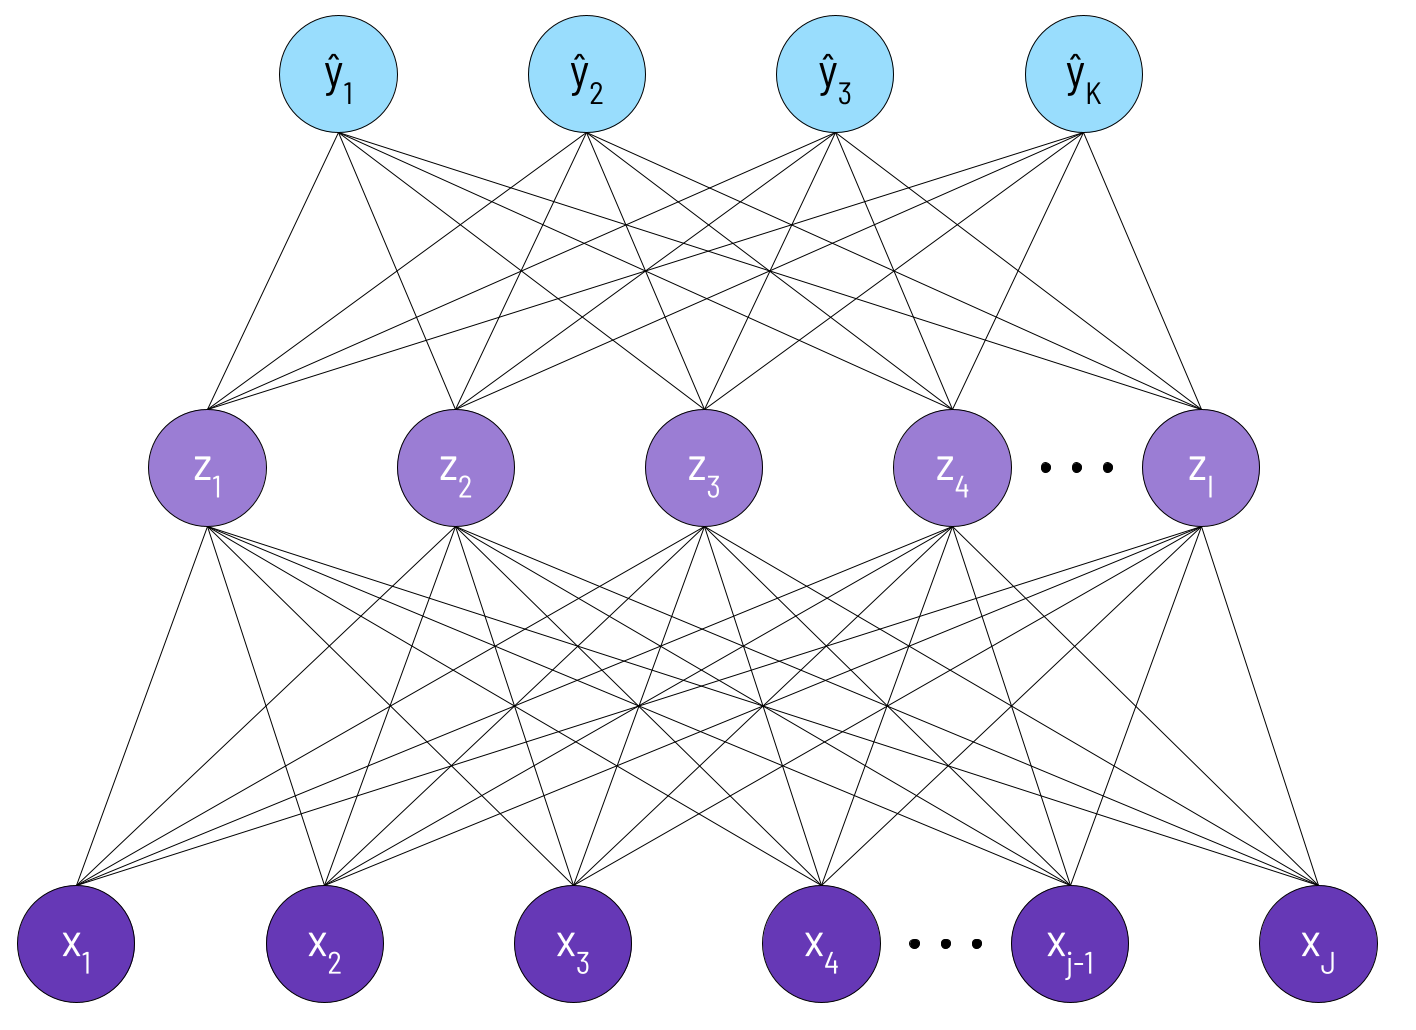
\includegraphics[width=\imgWidthL]{images/neural_network.png}
    \caption[One layered feed-forward network]{Feed forward network with one hidden layer. The illustration depicted is inspired by the schematic described in \cite{hastie2009elements}.}
    \label{neural_network}
\end{figure}
% Please add the following required packages to your document preamble:
% \usepackage[table,xcdraw]{xcolor}
% If you use beamer only pass "xcolor=table" option, i.e. \documentclass[xcolor=table]{beamer}
\begin{table}[H]
    \centering
    \begin{tabular}{|c|l|}
        \hline
        \rowcolor[HTML]{6638B6}
        {\color[HTML]{FFFFFF} Name} & \multicolumn{1}{c|}{\cellcolor[HTML]{6638B6}{\color[HTML]{FFFFFF} Formula}} \\ \hline
        Sigmoid                     & $\phi(z)=\frac{1}{1+e^{-z}}$                                                \\ \hline
        Tanh                        & $\phi(z)=\frac{e^{2z}-1}{e^{2z}+1}$                                         \\ \hline
        Relu                        & $\phi(z)=\max\{0,z\}$                                                       \\ \hline
    \end{tabular}
    \caption{List of some popular activation functions used in \acp{NN}}
    \label{tab:activation_functions}
\end{table}
Numerous activation functions are available for $\phi$, so the choice depends on data distribution, network architecture, task objective, and more \cite{DBLP:journals/corr/abs-1811-03378}. See \ref{tab:activation_functions} for a list of some popular activation functions. The ReLU activation function, for example, is widely used in hidden layers due to its simplicity and effectiveness \cite{DBLP:journals/corr/abs-2101-09957}\cite{DBLP:journals/corr/abs-2109-14545}. Generally, it is essential to add non-linearity to the \ac{NN} to make the model learn, represent and process any data and any arbitrary complex function to map inputs to outputs \cite{Sharma2020}, which on the other hand, requires minimizing an NP-hard high-dimensional non-convex objective \cite{NEURIPS2018_a41b3bb3}. This can be thought of as finding a global minimum in a chaotic, highly non-convex landscape as depicted in \figref{non_convex_landscape}.

\begin{figure}[H]%[htbp]
    \centering
    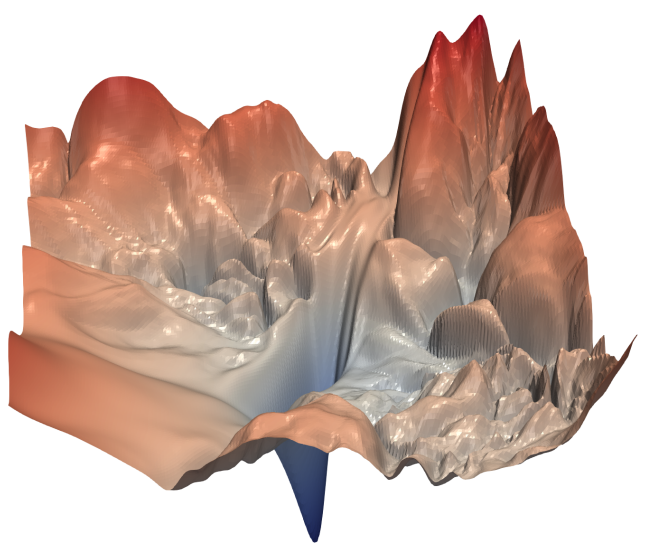
\includegraphics[width=\imgWidthM]{images/non_convex_landscape.png}
    \caption[Non-convex landscape of objective]{Highly non-convex landscape describing the complex objective of a Neural Network. The image is taken from \cite{NEURIPS2018_a41b3bb3}.}
    \label{non_convex_landscape}
\end{figure}
This section was a brief review of important \ac{SL} methods. As we can see from the definition of the \squote{empirical risk} \ref{eqn:empirical_risk}, all supervised methods require a model $h$, a set of labeled data, and some loss function typically chosen based on the task to solve, which can be a classification or regression task. Additionally, the equation \ref{eqn:empirical_risk} must be minimized, which leads to optimization theory briefly described in the next section.

\subsubsection*{Optimization}
\label{subsubsec:optimization}
As we need to minimize the \squote{empirical risk} as defined in \ref{eqn:empirical_risk} we can write the final objective as
\begin{equation}
    \mathop{\min}_{\theta} J(\theta) = \frac{1}{m}\sum_{i=1}^m l(h_{\theta}(x_i),y_i)
\end{equation}
which formally means that we want to find parameters $\theta$ that minimize the average losses of the training data.

The optimization techniques to solve this problem directly depend on the algorithm. While for some fundamental methods, such as linear regression, we can use analytic solutions, \ac{NN} requires an optimization technique called gradient descent which minimizes the objective by updating the parameters in the opposite direction of the gradient of the objective function concerning the parameters $\theta$ \cite{DBLP:journals/corr/Ruder16}. Intuitively we can think of trying to find a path to reach at least a local minimum on a non-convex surface as illustrated in \figref{non_convex_landscape}.

One of the most critical parameters in deep learning optimization is the learning rate, which controls the size of the steps taken during each iteration of the optimization process \cite{goodfellow2016deep}. A low learning rate can result in slower convergence, while a high learning rate might hinder finding an appropriate minimum. In practice, adaptive learning rate methods can automatically adjust the learning rate during training \cite{DBLP:journals/corr/abs-1212-5701}.

Gradient descent is a widely-used optimization method in deep learning, and numerous variants have been developed to improve its performance. One such variant is stochastic gradient descent (SGD), which estimates the gradient instead of calculating the true gradient. This approach often leads to faster convergence compared to traditional gradient descent \cite{bottou2012stochastic}.

\subsection{Unsupervised Learning}
\label{subsec:unsupervised_learning}
A prominent subject within \ac{ML} is \acp{UL}, which explores data to recognize inherent patterns without the guidance of predefined output labels. Two big fields of \ac{UL} are Clustering \cite{mcgregor2004flow} and Dimensionality Reduction \cite{sorzano2014survey}. Some applications of Clustering are \acp{RS} \cite{lu2012recommender}, \ac{CS} \cite{shakya2021big} and \ac{TM} \cite{perlich2014machine} and Dimensionality Reduction includes topics as \ac{FE} \cite{boutilier2009online} \ac{SD} \cite{vogelstein2014discovery} \ac{MC} \cite{fevry2018unsupervised} or \ac{BDV} \cite{keim2013big}. Numerous methods combine supervised with unsupervised techniques, such as semi-supervised, self-supervised, or weakly supervised. While semi-supervised learning uses labeled and unlabeled data, self-supervised learning attempts to generate labeled data independently, and weakly-supervised learning uses only partial information about the label \cite{9442775}. As this project focuses on \ac{SL} techniques, please refer to the keywords and papers mentioned above for further information.

\begin{figure}[H]%[htbp]
    \centering
    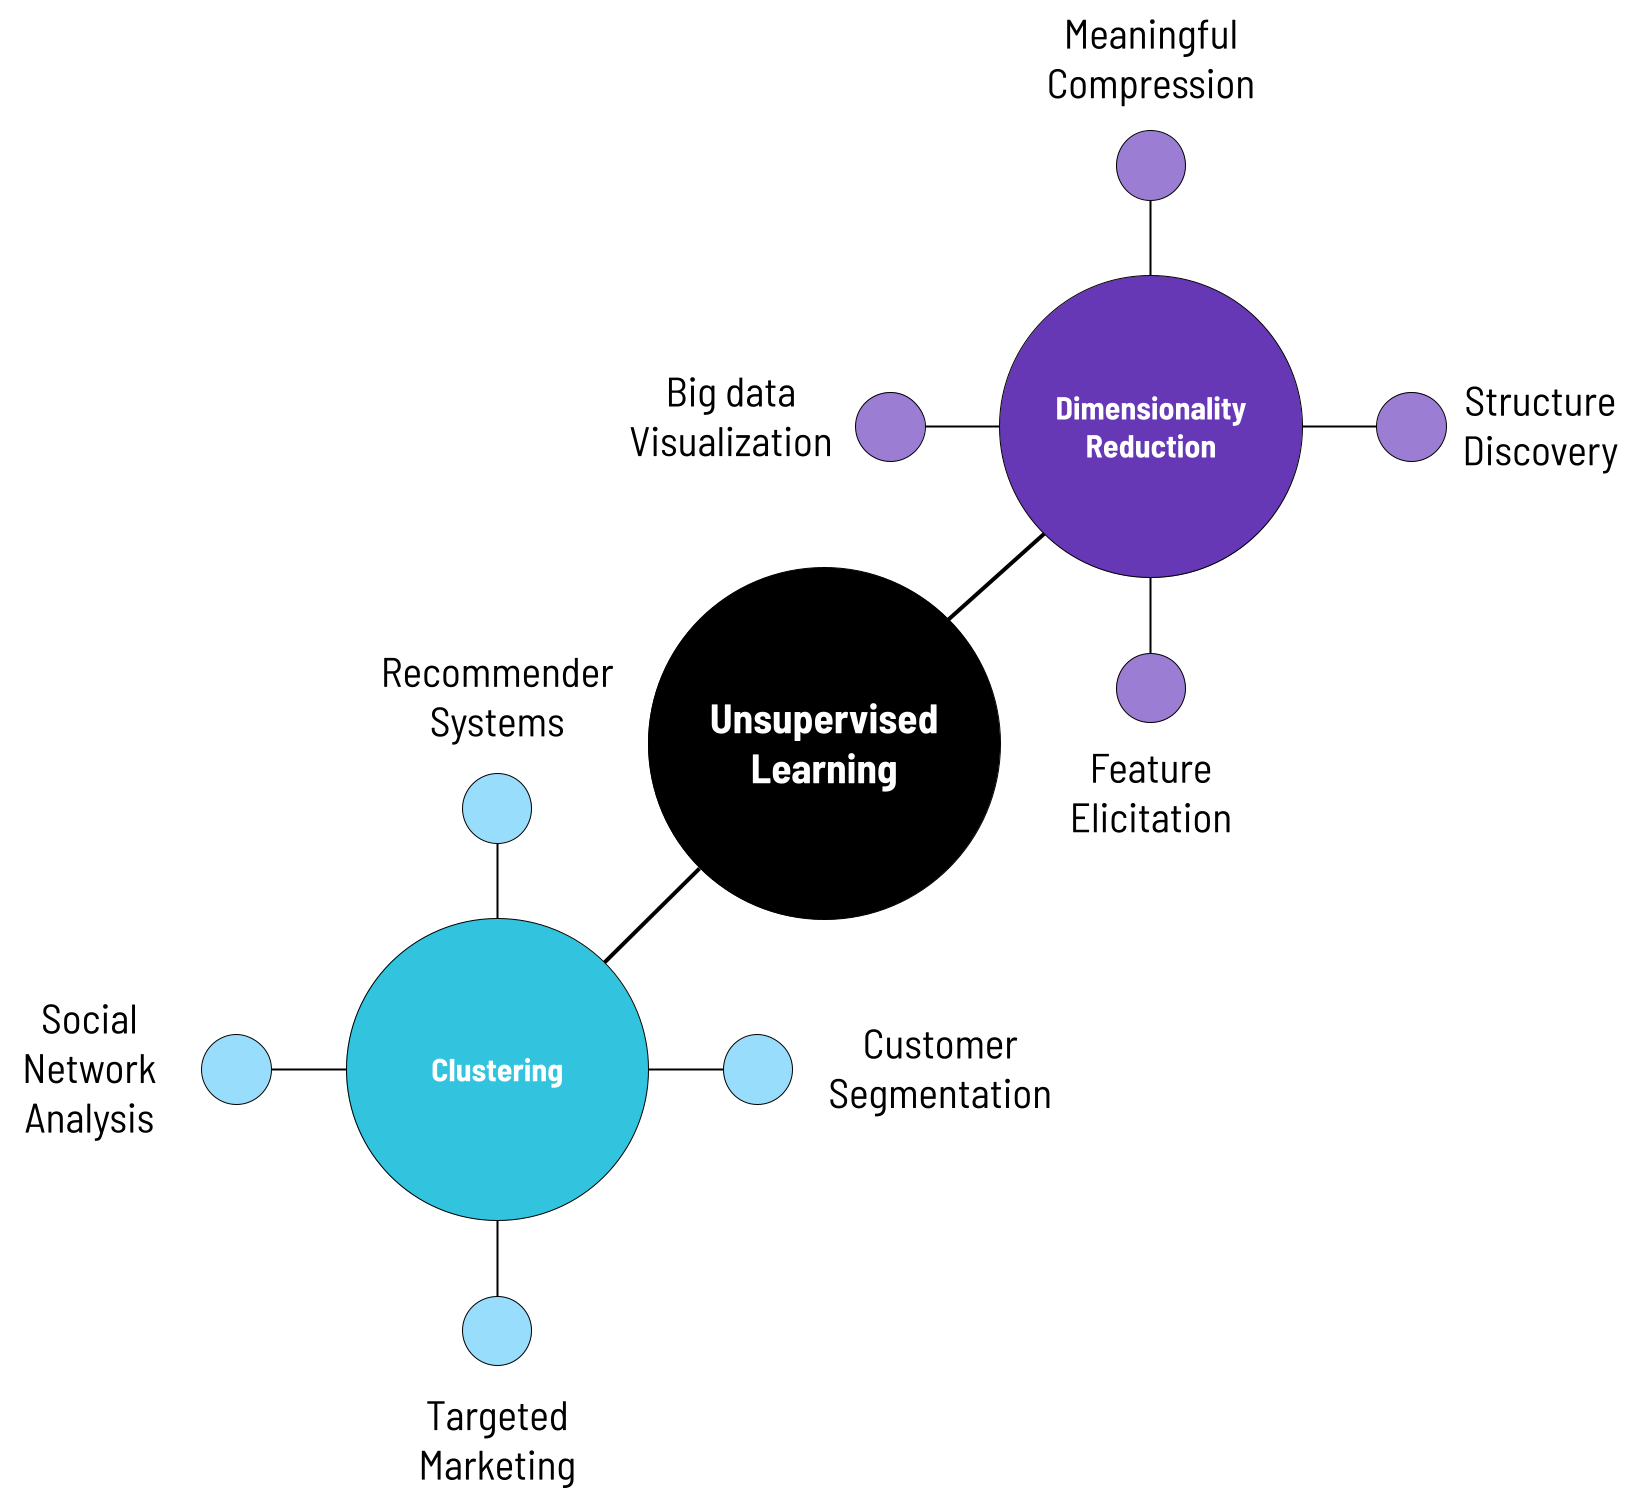
\includegraphics[width=\imgWidthM]{images/UnsupervisedLearning.png}
    \caption[Applications of \acf{UL}]{Applications of \acf{UL}. The image is inspired from \cite{unsupervisedLearning1}}
    \label{UnsupervisedLearning}
\end{figure}

\subsection{Reinforcement Learning}
Another large field of \ac{ML} is \acf{RL}, which relies on using training data to evaluate actions to take. In \ac{RL}, the correct action leads to the choice of subsequent actions. While the agent\footnote{The intelligent agent is a term used extensively in the literature. The book \cite{russel2010} defines \ac{AI} as the study of agents that receive percepts from the environment and perform actions.} is not told what actions to complete, it tries to discover what action can produce a maximum feedback signal also known as reward \cite{NIPS2013_e034fb6b}. \ac{RL}, therefore, is a trial-and-error mechanism that learns through feedback \cite{Jia2020ReviewOR}.

\figref{ReinforcementLearning} illustrates a typical concept of \ac{RL} with an agent connected to its environment via perception and action. On every step, the agent receives as input $i$ an indication of the current state of the environment. Subsequently, the agent selects an action $a$, which changes the state of the environment. This state transition is then communicated to the agent through a scalar reinforcement signal $r$. The goal for the agent is to choose actions that increase the long-run sum of values of the reinforcement signal \cite{Kaelbling1996May}.

Numerous algorithms correspond to \ac{RL}. Those include dynamic programming \cite{busoniu2017reinforcement}, Monte Carlo methods \cite{hammersley2013monte}, Q-Learning \cite{van2016deep}, TD-Learning \cite{van2013reinforcement} or Sarsa algorithms \cite{zou2019finite}.

An important domain where \ac{RL} can be applied is in robotics, where \ac{RL} can help how to grasp objects \cite{joshi2020robotic}, interact with humans \cite{akalin2021reinforcement} or other robots \cite{mataric1997reinforcement}, or navigate through difficult environments \cite{liu2020robot}. Another domain is finance, where \ac{RL} can assist in portfolio management \cite{jiang2017deep}, trading \cite{deng2016deep}, or risk management \cite{jiang2017deep}. \ac{RL} can further assist in healthcare with providing diagnosis \cite{kao2018context}, treatment recommendation \cite{gottesman2018evaluating}, drug discovery \cite{zhou2019optimization} or be used for surgical robots \cite{richter2019open}. In the gaming field, \ac{RL} can help create intelligent agents that can play games such as chess \cite{silver2018general}, Go \cite{silver2009reinforcement}, poker \cite{heinrich2016deep} or even video games \cite{shao2019survey}. Additionally, \ac{RL} can be applied to \ac{CV} tasks such as feature detection \cite{bueno2017hierarchical}, image segmentation \cite{sahba2006reinforcement}, object recognition \cite{paletta2000active} or tracking \cite{yun2017action}. \chapref{chap:literature_review} will describe in more detail of how \ac{RL} methods can improve segmentation results.

\begin{figure}[H]%[htbp]
    \centering
    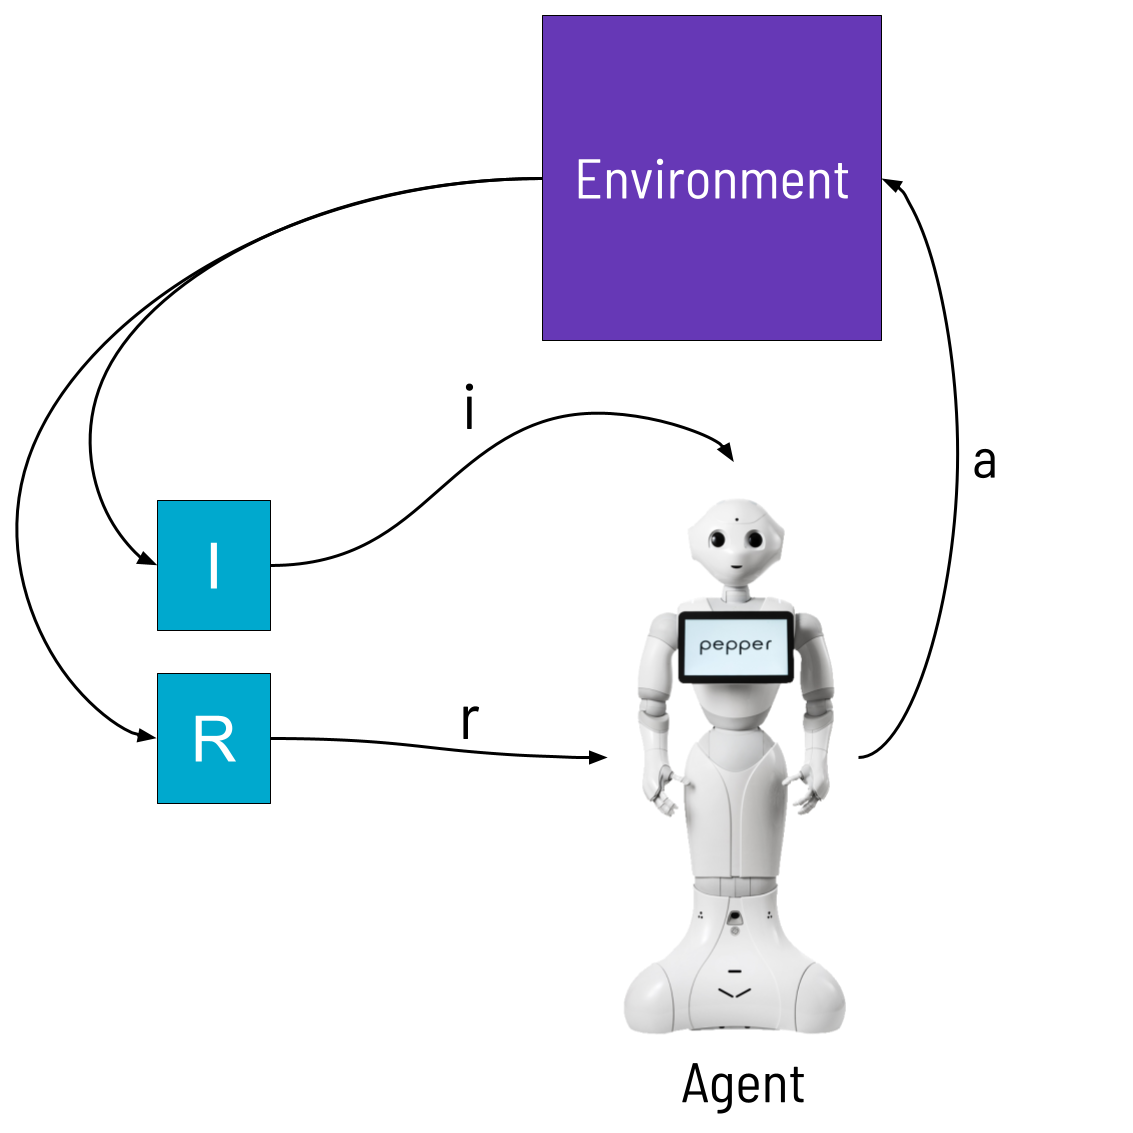
\includegraphics[width=\imgWidthM]{images/ReinforcementLearning.png}
    \caption[Concept of \acf{RL}]{Typical concept of \acf{RL} algorithm.}
    \label{ReinforcementLearning}
\end{figure}
\newpage

\begin{wrapfigure}{r}{0.4\textwidth}
    \centering
    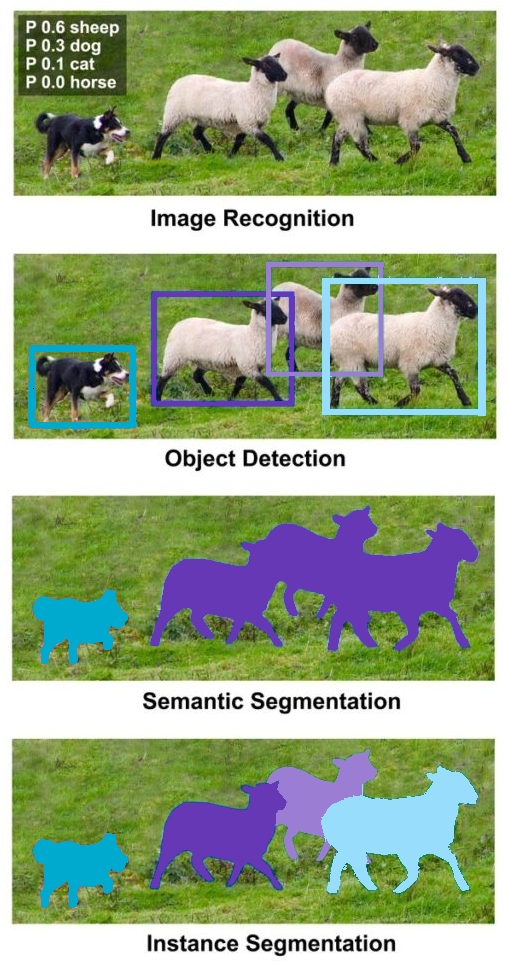
\includegraphics[width=0.30\textwidth]{images/semanticInstance_v1.jpg}
    \captionsetup{width=0.3\textwidth}
    \caption[Scene understanding]{Semantic segmentation within the context of scene understanding. Image from \cite{Bright2020Nov}.}
    \label{semanticInstance}
    \vspace{-20pt}
\end{wrapfigure}
\section{Semantic Segmentation}
This section offers a comprehensive overview of semantic segmentation using deep learning techniques. Semantic segmentation is a pixel-level classification algorithm that is crucial in comprehensively understanding images. According to \cite{GARCIAGARCIA201841}, many applications benefit from deriving insights from visual data. Notably, semantic segmentation has potential applications in a diverse range of fields, including but not limited to:

\begin{itemize}[noitemsep]
    \item Autonomous driving \cite{ess2009segmentation} \cite{feng2020deep} \cite{treml2016speeding} \cite{siam2018comparative} \cite{blum2019fishyscapes}
    \item Human-machine interaction \cite{oberweger2015hands}
    \item Computational photography \cite{yoon2015learning}
    \item Image search engines \cite{wan2014deep}
    \item Augmented reality \cite{ko2020novel} \cite{zhang2020slimmer}
    \item Medical imaging and diagnostics \cite{asgari2021deep} \cite{khan2021deep} \cite{du2020medical}
    \item Facial recognition \cite{meenpal2019facial} \cite{khan2015multi}
\end{itemize}

\figref{semanticInstance} illustrates four categories of scene understanding. \textit{Image recognition} provides a probability of objects detected within an image but does not give any information about their exact location. \textit{Object detection}, on the other hand, tries to locate and draw bounding boxes around every object in the image. \textit{Semantic segmentation} classifies pixels into preset categories. In the example shown, sheep and dogs are distinguished as separate categories. Finally, \textit{instance segmentation}, similar to semantic segmentation, can differentiate individual objects within the same class.
\subsection{Segmentation within Computer Vision}
As illustrated in \figref{AI_Overview}, semantic segmentation is a subfield of \acf{CV} and \acf{ML}. \ac{CV}, as a multidisciplinary field, encompasses a wide range of tasks and applications. Shapiro and Stockman define the objective of computer vision: \squote{The goal of computer vision is to make valuable decisions about real physical objects and scenes based on sensed images} \cite{shapiro2001computer}.

The authors describe Sensing, Encoded Information, Representations, and Algorithms as critical aspects of computer vision. \textit{Sensing} refers to how sensors acquire images and encode properties such as material, shape, illumination, and spatial relationships. \textit{Encoded Information} pertains to extracting information from images for a deeper understanding, including the geometry, texture, motion, or identity of objects. \textit{Representations} involve how images are represented for further use, considering their parts, properties, or relationships. \textit{Algorithms} describe the methods used to extract or process image information.\cite{shapiro2001computer}

\begin{figure}[H]%[htbp]
    \centering
    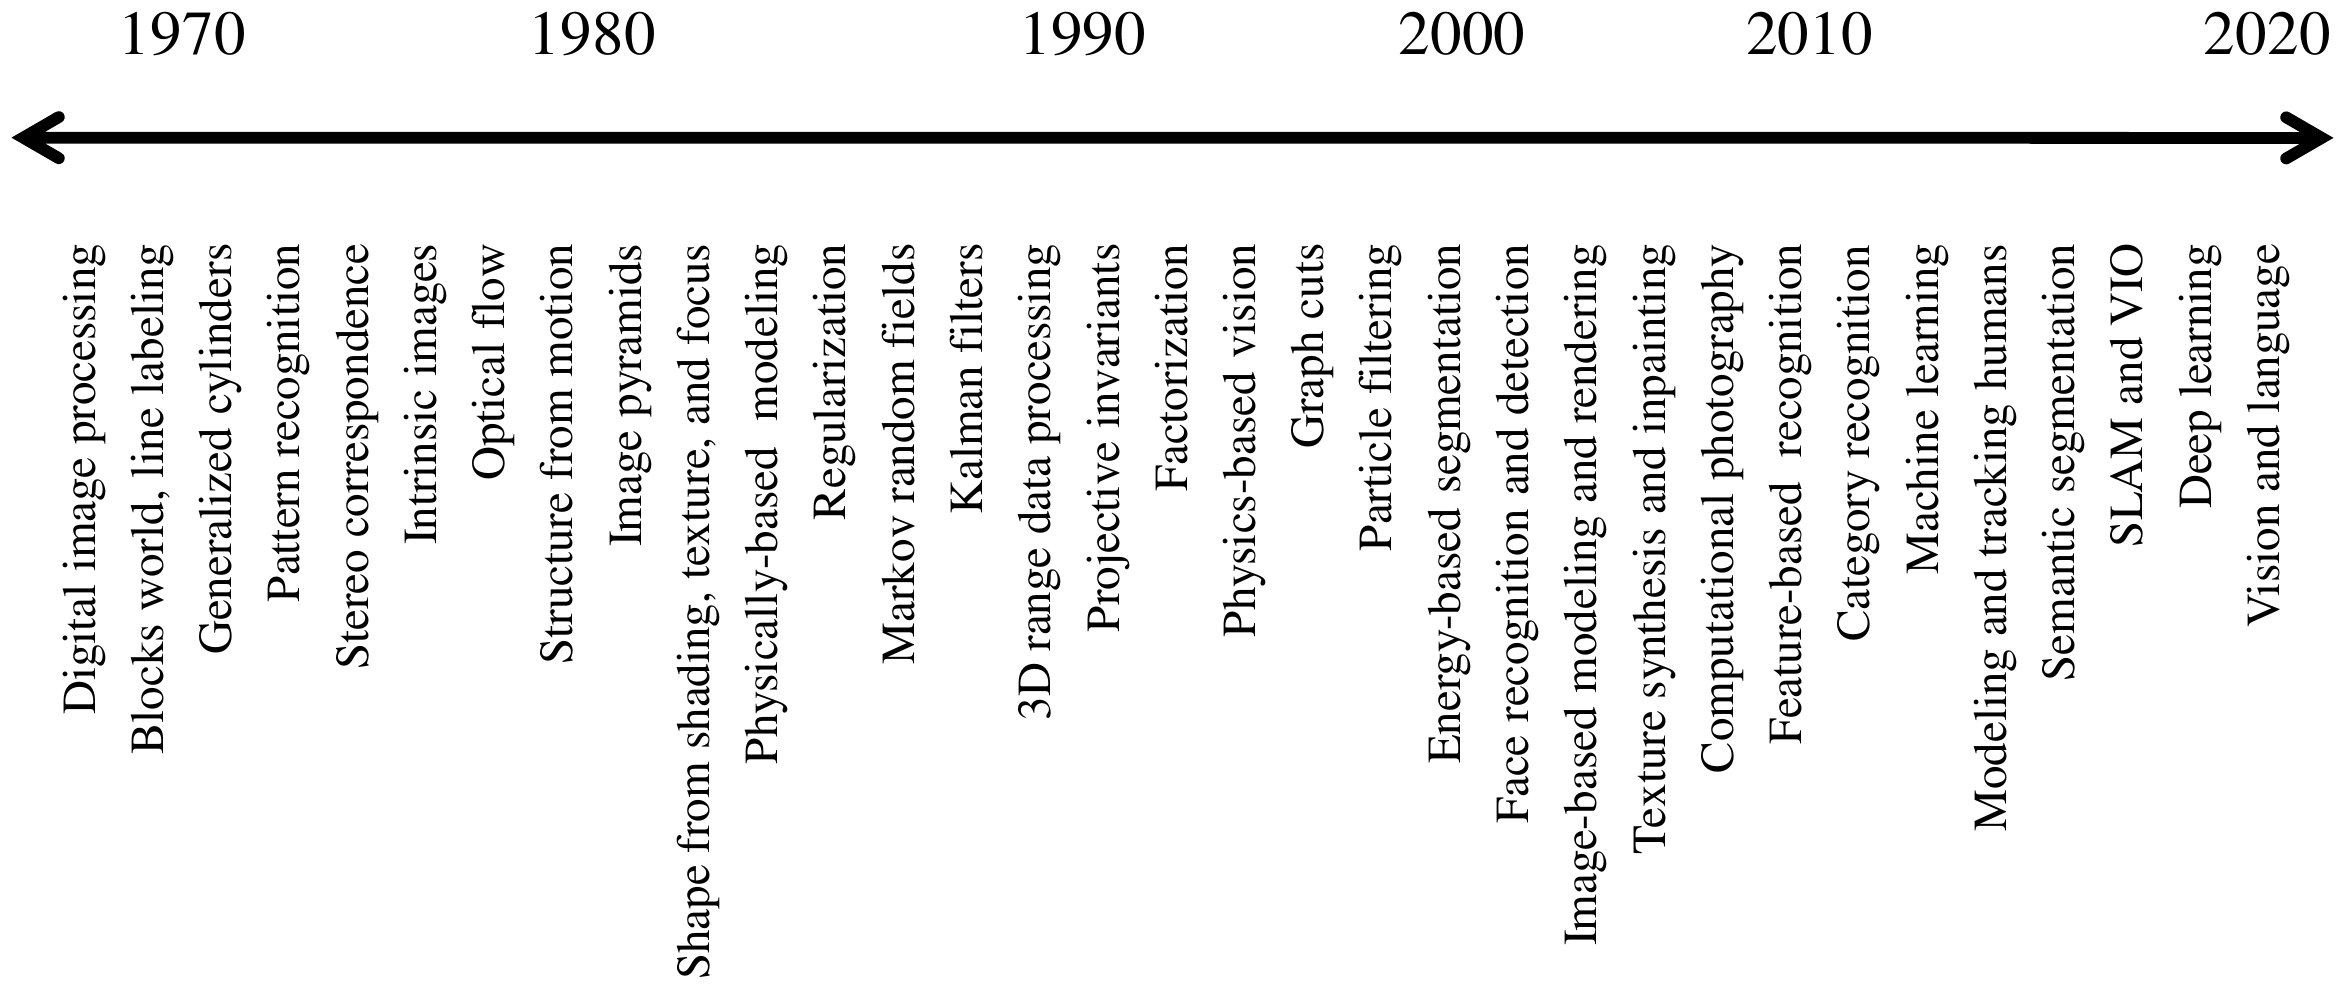
\includegraphics[width=\imgWidthXL]{images/timelineCV.png}
    \caption[Timeline of \acf{CV}]{Timeline of \ac{CV} research. Image from \cite{szeliski2022computer}}
    \label{timelineCV}
\end{figure}

Many algorithms used in computer vision were developed in studies dating back to the 1970s. \cite{szeliski2022computer} provides a fascinating timeline of the most important research topics in computer vision, as shown in \figref{timelineCV}. A significant breakthrough occurred in 2006 when Hinton introduced the Deep Belief Network with multiple layers of Restricted Boltzmann Machines. The author further states that the availability of large, public datasets and the advancement of parallel GPU computing contributed to the tremendous growth of deep learning.

The following chapter delves into some fundamental concepts of semantic segmentation, which, according to the timeline in \figref{timelineCV}, is a relatively new field within computer vision.

\subsection{Segmentation Objectives}
\label{subsec:segmentation_objectives}
As briefly mentioned above, and as illustrated in \figref{semanticInstance}, semantic segmentation aims to classify each pixel in an input image into a specific class. Applying the empirical risk introduced earlier to semantic segmentation, we have
\begin{equation}
    \mathop{\min}_{\theta} J(\theta) = \frac{1}{m}\sum_{i=1}^m l(h_{\theta}(x_i),y_i)
\end{equation}
where $m$ is the number of images in the dataset, $h_{\theta}$ the model, which typically consists of some form of \ac{CNN} architecture, $x$ the input image, $y$ the output label and $l$, the loss function which quantifies the difference between a prediction and the ground truth.

Numerous loss functions are suitable for semantic segmentation, which can be divided into different categories \cite{https://doi.org/10.48550/arxiv.2005.13449}. Subsequent sections offer an in-depth exploration of six notable loss functions, with two representatives from each category: distribution-based, region-based, and boundary-based, summarized in the following table \ref{tab:type_of_loss_functions_all}.
\begin{table}[H]
    \centering
    \begin{tabular}{|l|l|}
        \hline
        \rowcolor[HTML]{6638B6}
        {\color[HTML]{FFFFFF} \textbf{Types}} & {\color[HTML]{FFFFFF} \textbf{Names}}    \\ \hline
        Distribution-based                    & Cross-Entropy Loss (CE), Focal Loss (FL) \\ \hline
        Region-based                          & Dice Loss (DL), Tversky Loss (TL)        \\ \hline
        Boundary-based                        & Hausdorff Loss (HL), Boundary Loss (BL)  \\ \hline
    \end{tabular}
    \caption[Types of loss functions]{Types of loss functions}
    \label{tab:type_of_loss_functions_all}
\end{table}

\subsubsection*{Distribution-based}
Distribution-based loss functions focus on minimizing the dissimilarity of two distributions \cite{https://doi.org/10.48550/arxiv.2005.13449}. A principal loss function of this type is the \acf{CE}. Suppose a given segmentation task has two classes, we can use the \ac{BCE} derived from the Bernoulli distribution, and for a multi-class problem, we would use the \ac{CCE} derived from Multinoulli distribution \cite{Jadon_2020}.

\textbf{\acf{CE}}\newline
The binary cross-entropy loss can be formally defined as
\begin{equation}
    CE_{b}=-y\log(\hat{y})-(1-y)\log(1-\hat{y})
\end{equation}
For the case of multi-class classification, we would use the categorical cross-entropy loss defined as
\begin{equation}
    CE_{mc}=-\frac{1}{N}\sum_{i=1}^{N}\sum_{c=1}^C y_{i,c}\cdot \log(\sigma_{i,c})
    \label{eqn:CCE}
\end{equation}
where $N$ is the number of pixels, $C$ is the number of classes, and $\sigma_i$ is the normalized pixel with the softmax activation function as defined in \ref{eqn:softmax}.

The \ac{CE} or some variations are widely used for semantic segmentation. Prior studies claimed it works best in equal data distributions among classes \cite{Jadon_2020}. If the data is highly unbalanced, it can lead to the over-representation of larger objects in the loss, thus resulting in lower performance of smaller objects \cite{YEUNG2022102026}.

\textbf{\acf{FL}}\newline
\label{subsubsec:focal_loss}
The \ac{FL} \cite{lin2017focal} is a variant of the cross entropy loss. It provides excellent performance for highly imbalanced datasets by down-weighting easy examples and focusing on learning harder ones. The focal loss for binary classification is formally defined as
\begin{equation}
    FL_{b}=-\alpha(1-\hat{y}_t)^\gamma \cdot L_{BCE}
\end{equation}
and for multi-class classification as
\begin{equation}
    FL_{mc}=-\alpha(1-(\sigma_{i,c}))^\gamma \cdot L_{CCE}
\end{equation}
The $\alpha$ and $\beta$ parameters control how hard wrong predictions get penalized. \figref{focal_loss_plot} provides an example and the relation of \ac{FL} to \ac{CE}.

\begin{figure}[H]%[htbp]
    \centering
    \subfigure[]{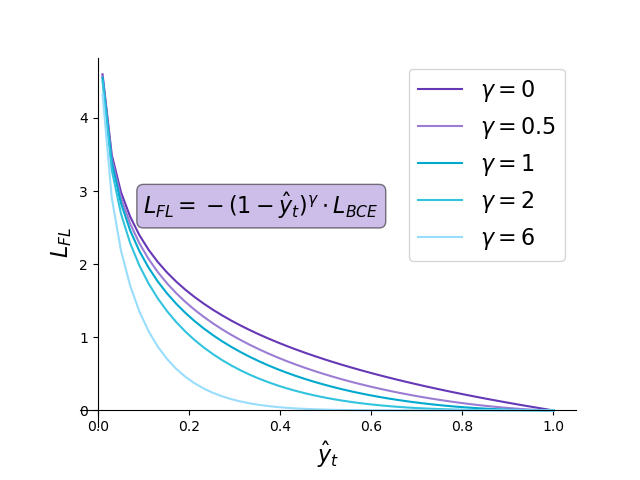
\includegraphics[width=\imgWidthTwo]{images/focal_loss_plot.png}}
    \subfigure[]{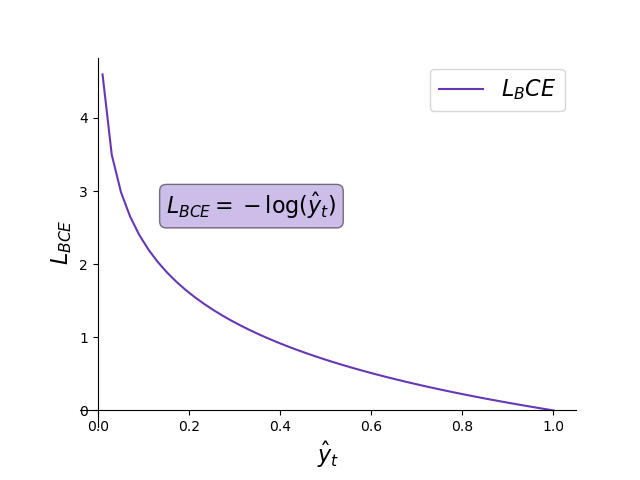
\includegraphics[width=\imgWidthTwo]{images/ce_loss_plot.png}}
    \caption[Graph of \acf{CE} and \acf{FL}]{\ac{FL} (a) as proposed in \cite{lin2017focal} with different values of $\gamma$. Whenever $\gamma=0$ focal loss turns into the regular \ac{CE} (b). Increasing $\gamma$ reduces the loss for well-classified examples, e.g., $\hat{y}_t > 0.6$ leading to a higher focus on misclassifications for hard examples.}
    \label{focal_loss_plot}
\end{figure}

\subsubsection*{Region-based}
\label{subsec:region_based}
Region-based loss functions primarily focus on the segmented regions within an image to ensure that the predicted output accurately captures the distinct areas or objects of interest. Region-based loss functions are also considered a prevalent type used in computer vision tasks such as semantic segmentation or object detection. The main difference between region-based and distribution-based loss functions is how they measure the difference between $\hat{y}$ and $y$. While region-based loss functions penalize incorrect classifications of individual pixels or regions, distribution-based loss functions penalize differences between the distribution of predicted class labels and ground truth labels.

\textbf{\acf{DL}}\\
\label{subsubsec:dice_similarity_coefficient_loss}
A popular region-based loss function for medical segmentation is the \acf{DL} based on the \ac{DSC}. The \ac{DSC} is defined as
\begin{equation}
    DSC= \frac{2|\hat{y} \cap y|}{|\hat{y}|+|y|}
    \label{eqn:dsc}
\end{equation}
where $\hat{y}$ is the set of predicted pixels and y the set of actual pixels. The numerator represents two times the cardinality of the intersection of the predicted and the actual set while the denominator is the sum of the predicted and actual cardinality.

As the \ac{DSC} is defined as a discrete set operation that is not differentiable \cite{9338261}, it cannot be directly used for training. To obtain a probabilistic version of the \ac{DSC}, an approximation known as the \ac{DL} was designed. The \ac{DL} penalizes the pixel-wise mismatch between a predicted map $\hat{y}$ and its corresponding ground truth $y$ for each class j. It is defined as
\begin{equation}
    DL=1-\frac{2\sum_{i=1}^P\sum_{j=1}^C y_{i,j} \hat{y}_{i,j}+\epsilon}{\sum_{i=1}^P\sum_{j=1}^C(y_{i,j}+\hat{y}_{i,j})+\epsilon}
\end{equation}
where $P$ is the number of pixels, $C$ the number of classes and $\epsilon$ a smoothing constant to avoid division by zero.

There are numerous variations of the dice loss. \cite{Sudre_2017} from 2017 introduces the \ac{GDL} which has the form
\begin{equation}
    GDL=1-2\frac{\sum_{l=1}^2 w_l\sum_{n y_{ln}\hat{y}_{ln}}}{\sum_{l=1}^2 w_l\sum_n y_{ln}+\hat{y}_{ln}}
    \label{eqn:gdl}
\end{equation}
where $w_l$ can provide invariance to specific label set properties by correcting the contribution of each label by the inverse of its volume. This technique can reduce the correlation between region size and dice score, which will be further discussed in \secref{sec:limiting_factors}.

\textbf{\acf{TL}}\newline
\label{subsubsec:tversky_loss}
\label{subsec:tversky}
The \ac{TL}, presented by \cite{DBLP:journals/corr/SalehiEG17a} was inspired by the Tversky index \cite{tversky1977features} from 1977 defined as
\begin{equation}
    S(\hat{y},y,\alpha,\beta)=\frac{|\hat{y} \cap y|}{|\hat{y} \cap y|+\alpha|\hat{y}\setminus y|+\beta|\hat{y}\setminus y|}
\end{equation}
where $\hat{y}$ and $y$ are sets of predicted and ground truth labels, respectively, and $\alpha$ and $\beta$ are hyperparameters that control the trade-off between false positives and false negatives.

The \ac{TL} aims to address the problem of high-precision, low-recall segmentations that can occur in highly imbalanced datasets. See \figref{precision_recall}. The authors claim this is an undesired property, especially in computer-aided diagnosis or clinical decision support systems where high recall is often more important than high precision.

The \ac{TL} is defined as follows:
\begin{equation}
    TL(\alpha,\beta)=\frac{\sum_{i=1}^N \sigma_{1i}y_{1i}}{\sum_{i=1}^N \sigma_{1i}y_{1i}+\alpha\sum_{i=1}^N \sigma_{1i}y_{0i}+\beta\sum_{i=1}^N \sigma_{0i}y_{1i}}
\end{equation}
where $\sigma_{0i}$ defined in \ref{eqn:softmax} is the probability of pixel $i$ to be part of the background region and $\sigma_{1i}$ the probability of pixel $i$ to be part of the foreground. $y_{1i}$ is 1 for a foreground pixel and $0$ for a background pixel. $y_{0i}$ would be 0 for a foreground pixel and $1$ for a background pixel. With $\alpha = \beta = 1$ the second term of the denominator would calculate the false positive rate and the second term the false negative rate. The hyperparameters $\alpha$ and $\beta$ control the balance between false positives and false negatives, with higher values of $\beta$ emphasizing false negatives and increasing recall.

\begin{figure}[H]%[htbp]
    \centering
    \subfigure[]{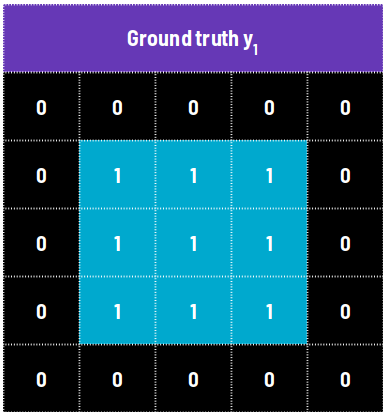
\includegraphics[width=\imgWidthFour]{images/tversky_high_precision_low_recall_y.png}}
    \subfigure[]{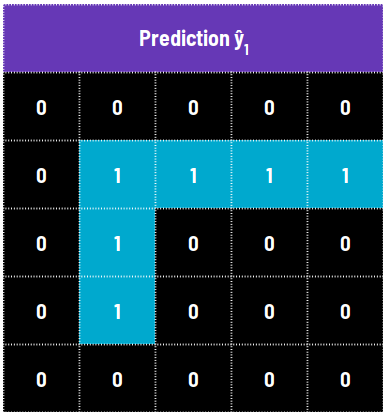
\includegraphics[width=\imgWidthFour]{images/tversky_high_precision_low_recall_yhat.png}}
    \subfigure[]{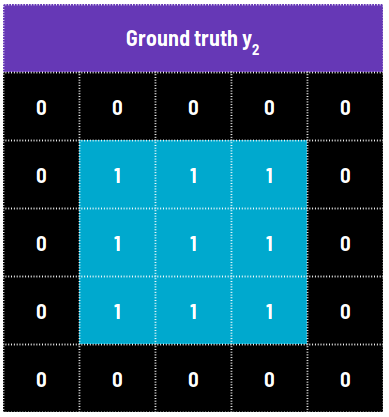
\includegraphics[width=\imgWidthFour]{images/tversky_low_precision_high_recall_y.png}}
    \subfigure[]{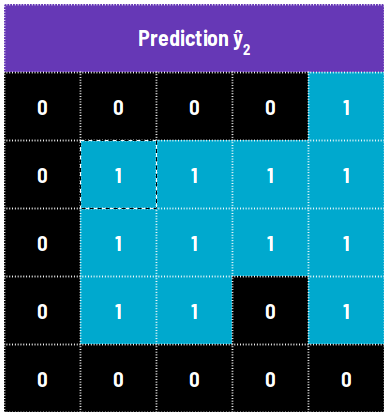
\includegraphics[width=\imgWidthFour]{images/tversky_low_precision_high_recall_yhat.png}}
    \caption[Precision and Recall]{Images (a) and (b) exhibit high precision $0.83$ with a low false positive rate and low recall $0.55$ with a high false negative rate, whereas images (c) and (d) show the opposite situation with low precision $0.61$ and a high false positive rate and high recall $0.88$ with a low false negative rate.  In heavily imbalanced datasets with a much smaller foreground class than the background class, it is common to encounter situations with high precision and low recall, resulting in many false negative classifications. This result is a critical problem in tasks such as medical image analysis, where detecting abnormalities is more important than achieving high precision \cite{powers2020evaluation}.}
    \label{precision_recall}
\end{figure}

\subsubsection*{Boundary-based}
\label{boundary_based}
Boundary-based loss functions represent a specialized type of loss functions that offers supplementary distance information, addressing the limitations of region-based and distribution-based loss functions. This section comprehensively analyzes two prominent boundary-based loss functions: \ac{BL} and \ac{HL}.

\textbf{\acf{HL}}\newline
\label{subsubsec:hausdorff_loss}
The Hausdorff loss was presented in the paper \squote{Reducing the Hausdorff Distance in Medical Image Segmentation with Convolutional Neural Networks}\cite{8767031} aiming to reduce an approximation of the \ac{HD}. The authors claim that the \ac{HD} is one of the most informative and useful objective criteria as an indicator for the largest segmentation error. The \ac{HD} was first introduced in the book called \squote{Grundz{\"u}ge der Mengenlehre} by Felix Hausdorff in the year 1914. Applied to the definitions of $y$ and $\hat{y}$ presented in \secref{sec:terminology}, defining their corresponding boundaries as $Y_b$ and $\hat{Y}_b$ the calculation for the one-sided \ac{HD} from the pointset $\hat{Y}_b$ to $Y_b$ is defined as follows \cite{rockafellar2009variational}:
\begin{equation}
    hd(\hat{Y}_b,Y_b)=\mathop{\max}_{\hat{y}_b \in \hat{Y}_b}\mathop{\min}_{y_b \in Y_b}||\hat{y}_b - y_b||_2
\end{equation}
and from the set $Y_b$ to $\hat{Y}_b$ as
\begin{equation}
    hd(Y_b,\hat{Y}_b)=\mathop{\max}_{y_b \in Y_b}\mathop{\min}_{\hat{y}_b \in \hat{Y}_b}||\hat{y}_b - y_b||_2
\end{equation}
\begin{figure}[H]%[htbp]
    \centering
    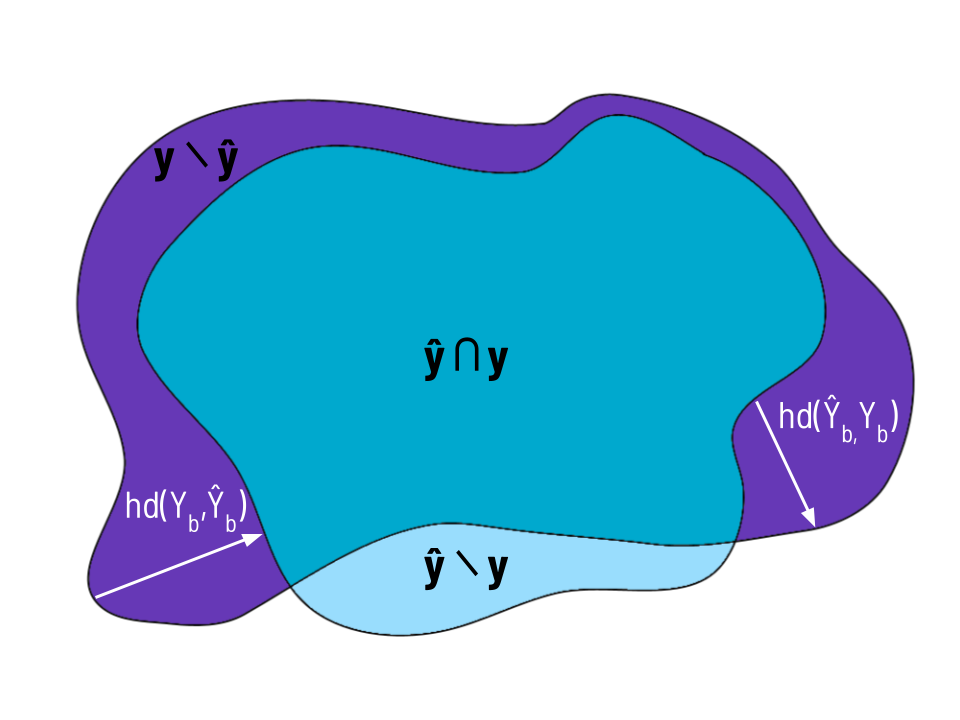
\includegraphics[width=0.5\textwidth]{images/Hausdorff_distance.png}
    \caption[Hausdorff distance]{Visual concept of the Hausdorff distance and some related notation. The two distances $hd(\hat{Y}_b,Y_b)$ and $hd(Y_b,\hat{Y}_b)$ represent the two largest segmentation errors from both the prediction boundary and output label boundary perspective. The contour additionally displays \textbf{\textcolor{rwucyan40}{false positives}} as $\hat{y}\setminus y$, \textbf{\textcolor{rwuviolet}{false negatives}} as $y\setminus\hat{y}$ and \textbf{\textcolor{rwucyan}{true positives}} as $\hat{y}\cap y$. The image is inspired by the visuals of \cite{8767031}}
    \label{Hausdorff_distance}
\end{figure}
When calculating $hd(\hat{Y}_b,Y_b)$, we can intuitively say that for every point $\hat{y}_{b,i}$ on the boundary $\hat{Y}$ we calculate the closest distance to the boundary $Y_b$ and then chose the largest value from all those closest distances. As we can see in the \figref{Hausdorff_distance}, $hd(y_b,\hat{y}_b)\neq hd(\hat{y}_b,y_b)$ which should be true in most cases. A bidirectional version of \ac{HD}, is defined as \cite{8767031}:
\begin{equation}
    HD(Y_b,\hat{Y}_b)=\max(hd(\hat{Y}_b,Y_b),hd(Y_b,\hat{Y}_b))
    \label{eqn:hd_bidirectional}
\end{equation}

The calculation of the \ac{HD} for segmentation purposes is shown to be done with the help of the distance transform method \cite{8767031}. The distance transform technique calculates the distance to a curve or a set of points using a two-pass raster algorithm \cite{szeliski2022computer}. Adjusted to the notation of the current work, the formal definition for the distance transform applied to the prediction $\hat{y}$ is defined as:
\begin{equation}
    D_{\hat{y}}(i,j)=\mathop{\min}_{k,l\:\hat{y}[k,l]=1} d(i-k,j-l)
    \label{eqn:distance_transform_yhat}
\end{equation}
or for $y$ as
\begin{equation}
    D_{y}(i,j)=\mathop{\min}_{k,l\:y[k,l]=1} d(i-k,j-l)
    \label{eqn:distance_transform_y}
\end{equation}
Note that we assume that the input, whether from $y$ or $\hat{y}$, is provided as a binary image. The equations \ref{eqn:distance_transform_yhat} and \ref{eqn:distance_transform_y} calculate the distance for every pixel to the nearest pixel with the value 1. \figref{hausdorff_dt} provides an example calculation for $D_{\hat{y}}(i,j)$ and $D_{y}(i,j)$ with input shape of $([1,1,5,5])$ for $y$ and $\hat{y}$.

\begin{figure}[H]%[htbp]
    \centering
    \subfigure[]{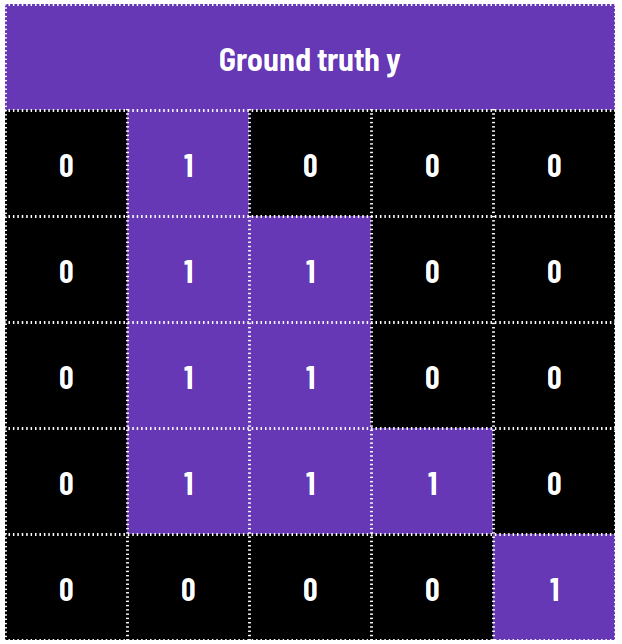
\includegraphics[width=\imgWidthFour]{images/hausdorff_y.png}}
    \subfigure[]{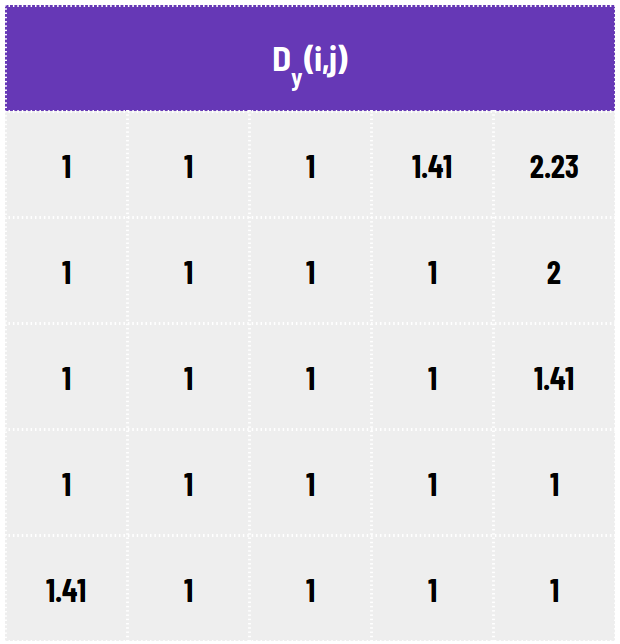
\includegraphics[width=\imgWidthFour]{images/hausdorff_dt_y.png}}
    \subfigure[]{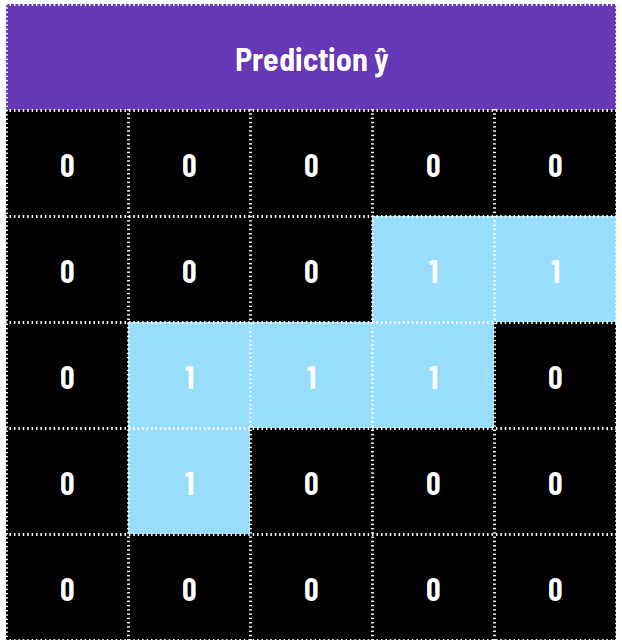
\includegraphics[width=\imgWidthFour]{images/hausdorff_yhat.png}}
    \subfigure[]{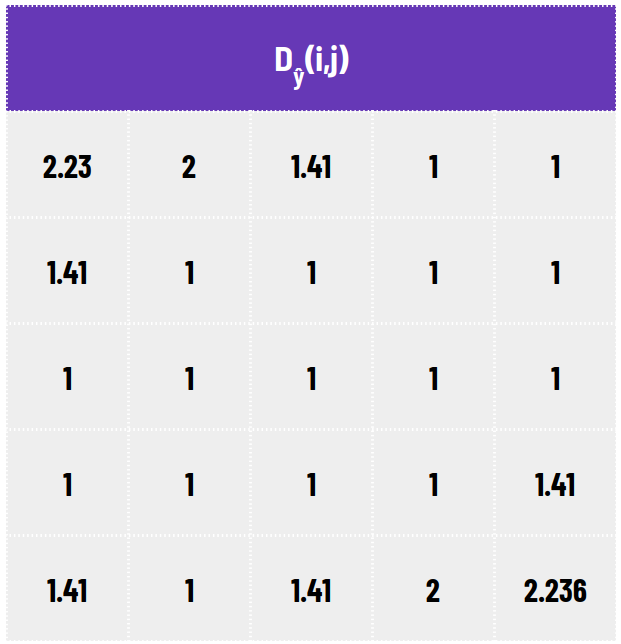
\includegraphics[width=\imgWidthFour]{images/hausdorff_dt_yhat.png}}
    \caption[Distance transform calculation]{Distance transform calculation for ground truth $y$ (a) and $\hat{y}$ (c). We can see that $D_y$ (b) and $D_{\hat{y}}$ (d) contain values that consist of distances. The position of these distances corresponds to the same position of the input $y$ and $\hat{y}$ and the distances indicate how far this pixel was from the closest pixel with the value 1.}
    \label{hausdorff_dt}
\end{figure}
For the final calculation of the \ac{HD} for segmentation, we first have to subtract $y$ from $\hat{y}$ or vice versa and then take the absolute value from the result. We still input the binary maps of $y$ and $\hat{y}$. The result will highlight false positives and false negatives as a new binary map defined as $|y-\hat{y}|$ or in set notation $y\setminus\hat{y}\cup\hat{y}\setminus y$. See \figref{hausdorff_y_minus_yhat}  or \figref{Hausdorff_distance} for further information. To finalize we need calculate $hd_D(Y_b,\hat{Y}_b)$ as
\begin{equation}
    hd_D(Y_b,\hat{Y}_b)=\mathop{\max}_{\Omega}(|y-\hat{y}|\circ D_{\hat{y}}(i,j))
\end{equation}
and $hd_D(\hat{Y}_b,Y_b)$ as
\begin{equation}
    hd_D(\hat{Y}_b,Y_b)=\mathop{\max}_{\Omega}(|y-\hat{y}|\circ D_{y}(i,j))
\end{equation}
The subscript $D$ on $hd_D$ indicates that we use the distance transform for this type of calculation. $\circ$ stands for the Hadamard product, an element-wise product of two matrices of the same size \cite{horn1990hadamard}. $\Omega$ represents the grid where the image is established, indicating that the maximum value pertains to all the pixels. \figref{hausdorff_y_minus_yhat} provides the result of the example calculation from above. For the bidirectional version, we could take \ref{eqn:hd_bidirectional} as the final loss definition.
\begin{figure}[H]%[htbp]
    \centering
    \subfigure[]{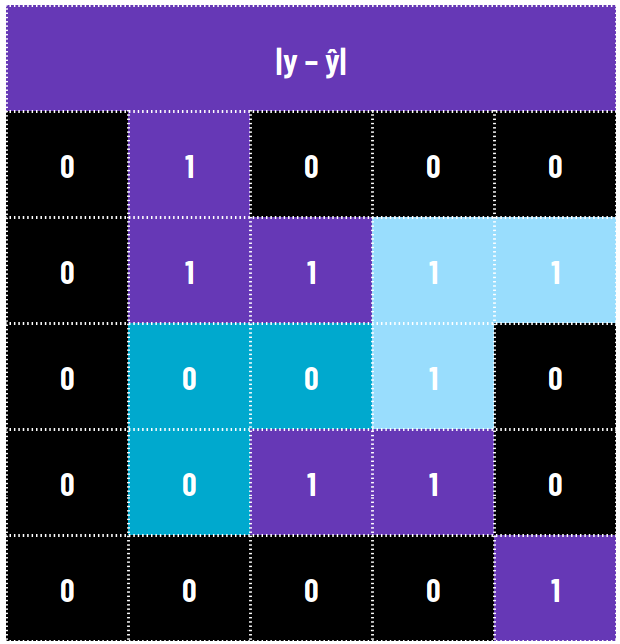
\includegraphics[width=\imgWidthThree]{images/hausdorff_y_minus_yhat.png}}
    \subfigure[]{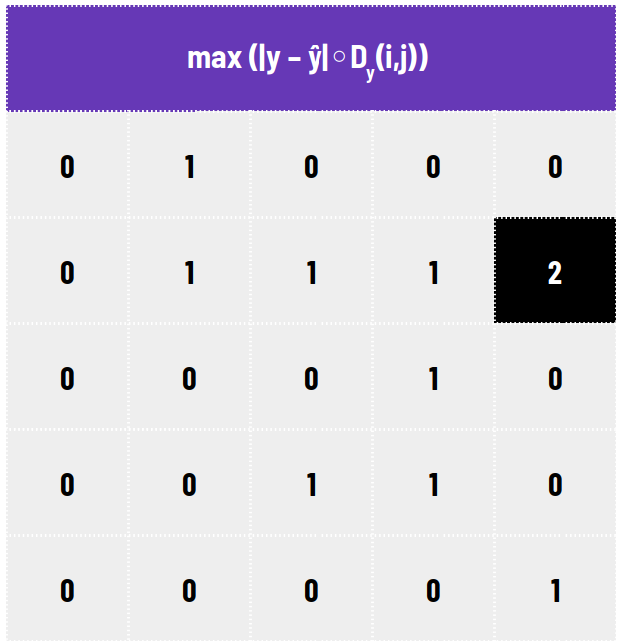
\includegraphics[width=\imgWidthThree]{images/hausdorff_max_y.png}}
    \subfigure[]{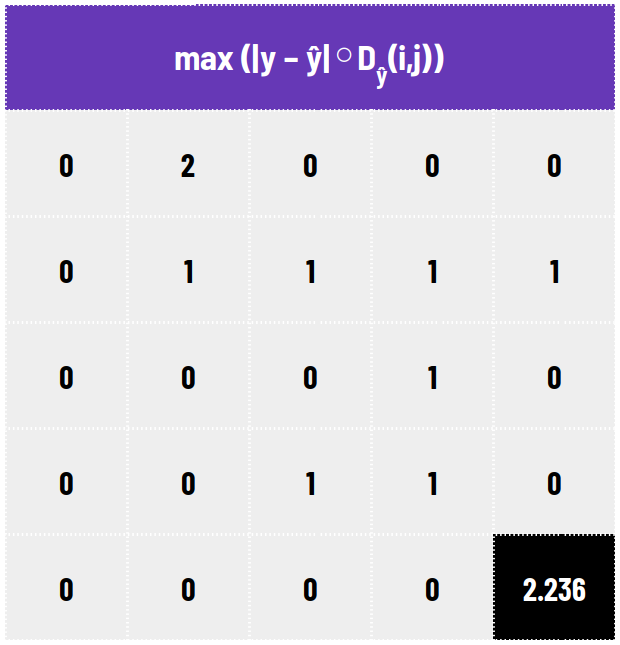
\includegraphics[width=\imgWidthThree]{images/hausdorff_max_yhat.png}}
    \caption[Hausdorff calculation result]{Image (a): \textbf{\textcolor{rwuviolet}{False negatives}}: Values predicted mistakenly as zero. \textbf{\textcolor{rwucyan40}{False positives}}: Values predicted mistakenly as 1. \textbf{\textcolor{rwucyan}{True positives}}: Correctly predicted values.The values containing one can also be described in set notation as $y\setminus\hat{y}\cup\hat{y}\setminus y$. Image (b-c): Result of the final calculation of $hd_D(Y_b,\hat{Y}_b)$ and $hd_D(\hat{Y}_b,Y_b)$.}
    \label{hausdorff_y_minus_yhat}
\end{figure}
Even if reducing the \ac{HD} directly sounds plausible, the definition \ref{eqn:hd_bidirectional} has some drawbacks. The authors of \cite{8767031} describe some disadvantages due to the limited focus on the largest distance between the boundaries, which can lead to unstable behavior in other regions. The paper refers to other works that attempted to use the \ac{HD} where most studies focus on restricted tasks such as face detection or object matching. To improve stability by focusing on the entire region of $y\setminus\hat{y}\cup\hat{y}\setminus y$, the paper proposes the following loss:
\begin{equation}
    HL(\hat{y},y)=\frac{1}{|\Omega|}\sum_{\Omega}((y-\hat{y})^2\circ (D_y^{\alpha} + D_{\hat{y}}^{\alpha}))
    \label{eqn:hausdorff_loss}
\end{equation}
which smoothly penalizes larger segmentation errors but takes the entire boundary into account. The parameter $\alpha$ determines how strongly large errors are getting penalized.

A proposed alternative for this project, where instead of raising the distance transform $D_y$ and $D_{\hat{y}}$ to the power of the hyperparameter $\alpha$ and then adding both values, uses the absolute values of their sum to guarantee the necessary positive values while providing a lower weight on the right factor of the equation above, is additionally suggested after providing promising results after some initial tests. Formally, this variant is defined as
\begin{equation}
    HL_{1}(\hat{y},y)=\frac{1}{|\Omega|}\sum_{\Omega}((y-\hat{y})^2\circ |D_y + D_{\hat{y}}|)
    \label{eqn:hausdorff_loss_v2}
\end{equation}

Another disadvantage is the high computational cost for $D_{\hat{y}}(i,j)$. It cannot be precalculated as $D_{y}(i,j)$ as the prediction $\hat{y}$ changes during training. The paper, therefore, suggests a \squote{one-sided} alternative defined as:
\begin{equation}
    HL_{os}=(y,\hat{y})=\frac{1}{\Omega}\sum_{\Omega}((y-\hat{y})^2\circ D_y^{\alpha})
    \label{eq:one_sided_hd}
\end{equation}

\textbf{\acf{BL}}\newline
\label{subsubsec:boundary_loss}
The paper \squote{Boundary loss for highly unbalanced segmentation}\cite{Kervadec_2021} introduces a new \acp{BL}. The general goal of the paper is to face the problems of unbalanced segmentation, which is relatively common in medical image analysis. The suggested boundary loss is supposed to provide additional information complementary to regional losses. The authors claim that the main challenge is building a differentiable function considering the regions between $Y_b$ and $\hat{Y}_b$. Those regions are equivalent to $y\setminus\hat{y}\cup\hat{y}\setminus y$, which consists of the union of false negatives and false positives. From now on, we define $\Delta S=y\setminus\hat{y}\cup\hat{y}\setminus y$, which is equivalent to the union of the \textcolor{rwuviolet}{dark violet} and \textcolor{rwucyanlight}{light cyan regions} in \figref{Hausdorff_distance}.
\begin{figure}[H]%[htbp]
    \centering
    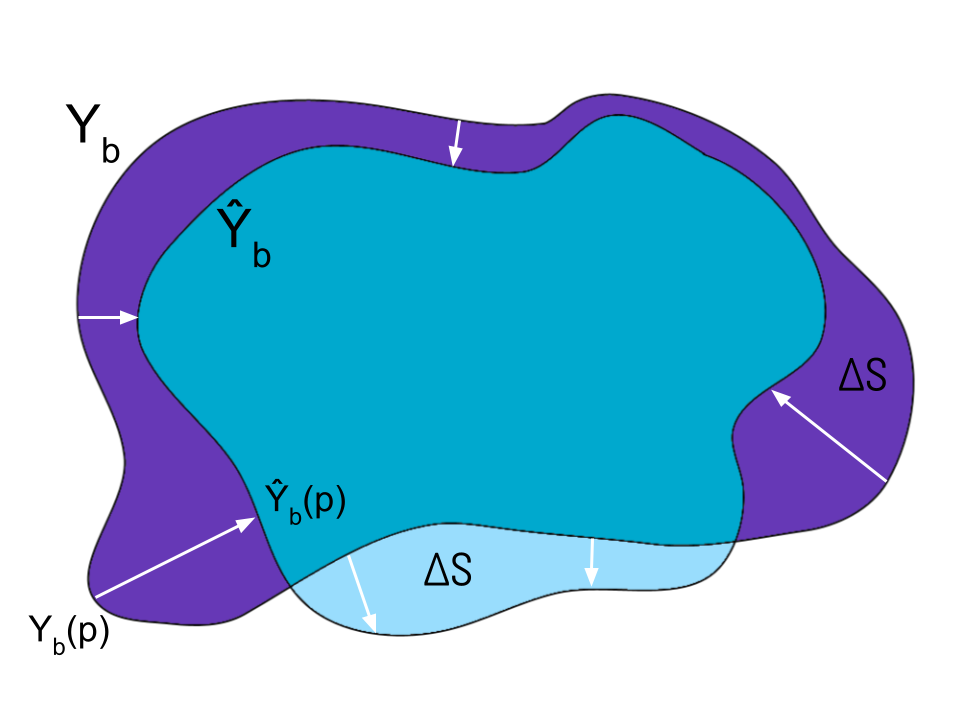
\includegraphics[width=0.5\textwidth]{images/BoundaryDiff.png}
    \caption[Boundary normals]{Schematic representation of the normals indicated as white arrows perpendicular to $Y_b$ at $Y_b(p)$ and its intersection at $\hat{Y}_b(p)$.}
    \label{BoundaryDiff}
\end{figure}
The loss proposed in \cite{Kervadec_2021} is inspired by graph-based optimization techniques \cite{boykov2006integral} and attempts to approach
\begin{equation}
    Dist(Y_b,\hat{Y}_b)=\int_{Y_b}||Y_b(p)-\hat{Y}_b(p)||^2 dp
    \label{eqn:boundary_diff}
\end{equation}
with
\begin{equation}
    Dist(Y_b,\hat{Y}_b)\approx 2\int_{\Delta S}D_y(q)dq
\end{equation}
where $Y_b(p)$ and $\hat{Y}_b(p)$ denote two corresponding points on the boundary connected by the normal to $Y_b$ at $p$ and its intersection $\hat{Y}_b(p)$. See \figref{BoundaryDiff}. As the expression \ref{eqn:boundary_diff} cannot be directly used for a loss due to local differential computations of the normal \cite{Kervadec_2021}, it can be approximated using the distance transform $D_y(q)$ where $q$ refers to any pixel on the ground truth $y$. The distance transforms $D_y(q)$, therefore, calculates the distance from $q$ to the closest point on the boundary $Y_b$.

The final loss is then calculated based on a level set representation \footnote{A level set representation is a method of representing objects and boundaries in a computer simulation or image processing using a level set function. The level set function assigns a numerical value to each point in a given space, such as an image or a three-dimensional model. Points inside or on the boundary have one value, while points outside the object have another. The points where the value of the function changes from one to another are called level sets. They are the contours of the object or the boundary.} $\varphi_y(q)$ which is calculated from the distance transform $D_y(q)$ as:
\begin{equation}
    \varphi_y(q)
    \begin{cases}
        -D_y(q) & \text{if }q\in y \\
        D_y(q)  & \text{otherwise}
    \end{cases}
    \label{eqn:varphi}
\end{equation}

\begin{figure}[H]%[htbp]
    \centering
    \subfigure[]{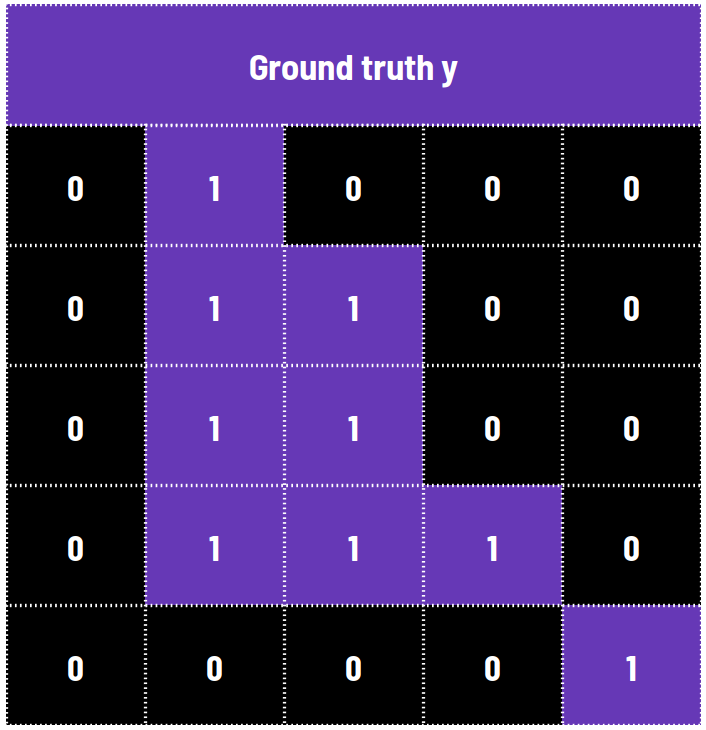
\includegraphics[width=\imgWidthThree]{images/varphi_q_1.png}}
    \subfigure[]{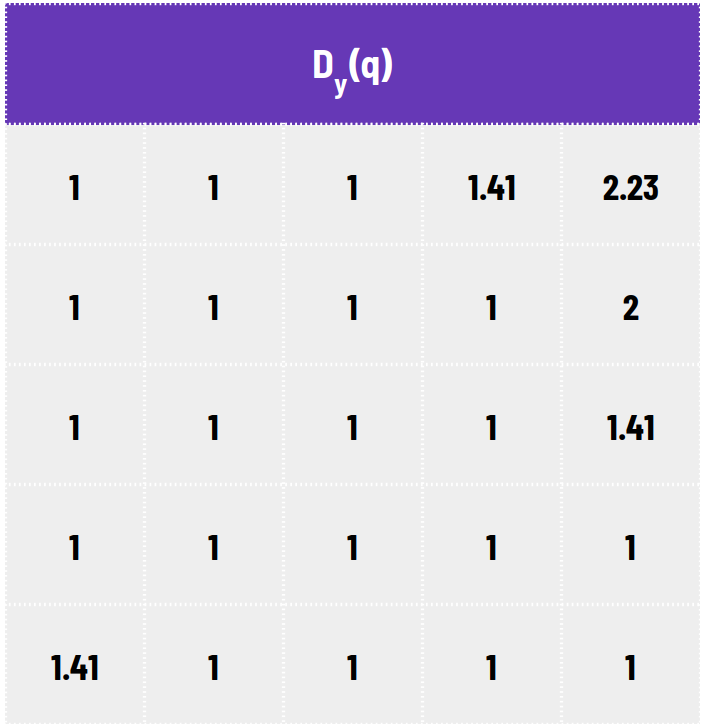
\includegraphics[width=\imgWidthThree]{images/varphi_q_2.png}}
    \subfigure[]{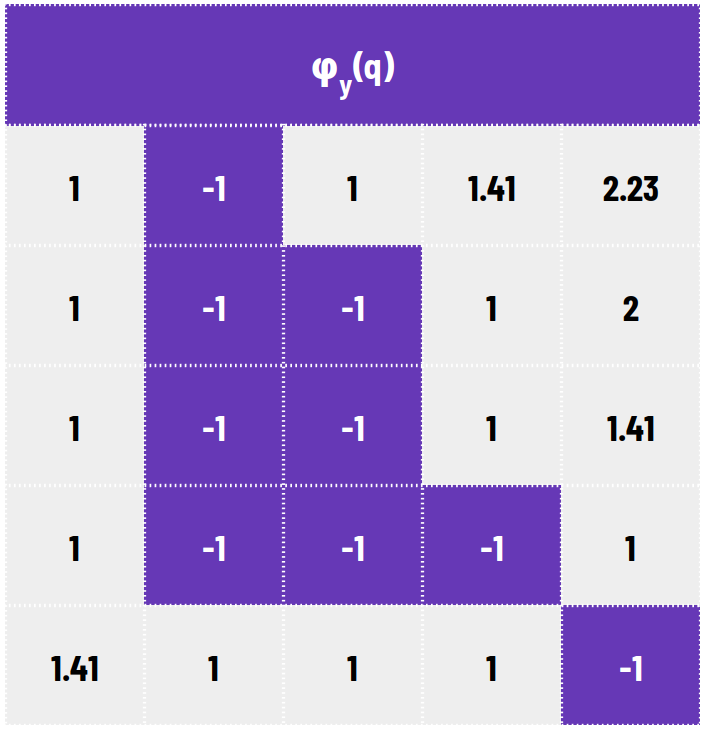
\includegraphics[width=\imgWidthThree]{images/varphi_q_3.png}}
    \caption[Calculation of $\varphi_y(q)$]{Example calculation of $\varphi_y(q)$ (c) from $y$ (a) with equation $\ref{eqn:varphi}$. Image (b) depicts the distance transform $D_y(q)$.}
    \label{varphi_q}
\end{figure}
which then leads to
\begin{equation}
    Dist(Y_b,\hat{Y}_b)=\int \varphi_y(q)\hat{y} dq -\int \varphi_y(q)y dq=BL
\end{equation}
which has the major advantage that the level set function $\varphi_y(q)$ can be precomputed from the ground truth as it does not change during training.
\begin{figure}[H]%[htbp]
    \centering
    \subfigure[]{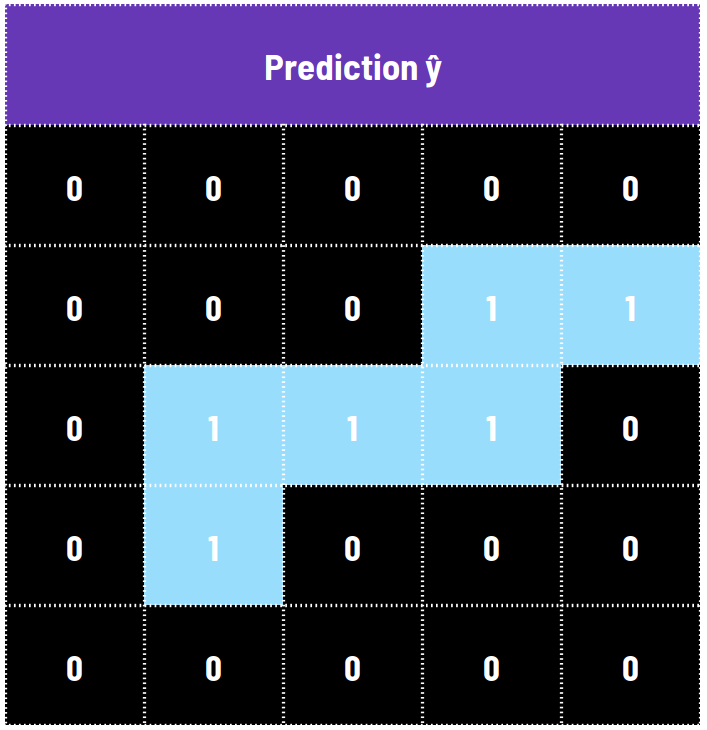
\includegraphics[width=\imgWidthFour]{images/boundary_final_1.png}}
    \subfigure[]{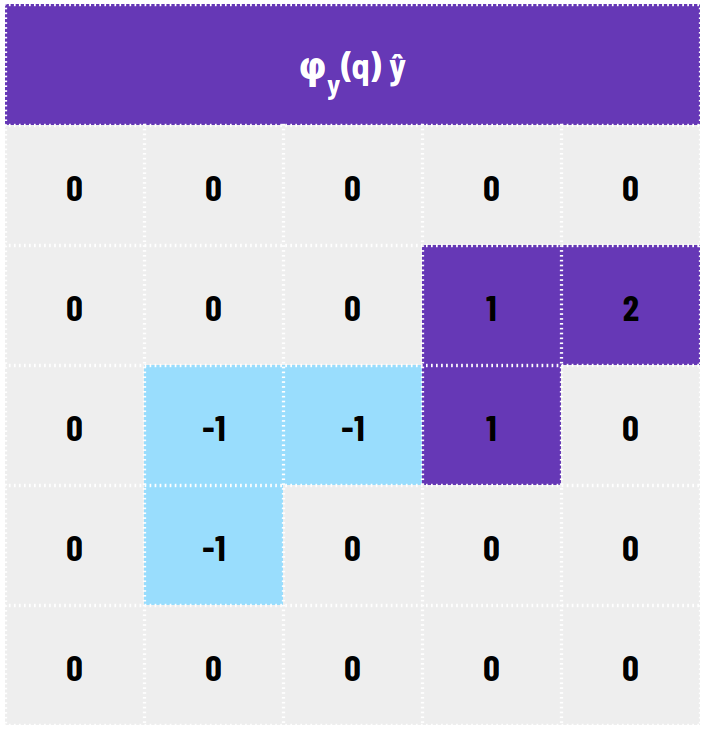
\includegraphics[width=\imgWidthFour]{images/boundary_final_2.png}}
    \subfigure[]{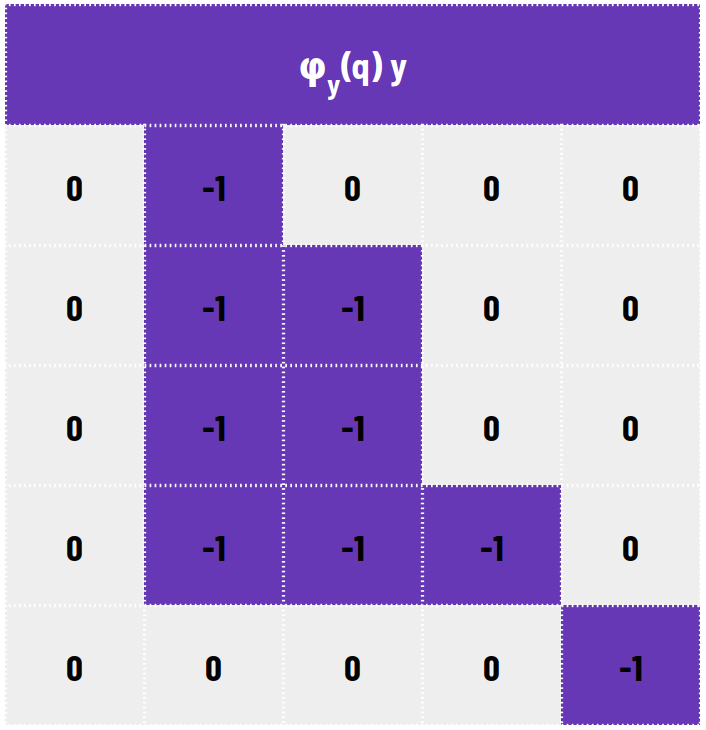
\includegraphics[width=\imgWidthFour]{images/boundary_final_3.png}}
    \subfigure[]{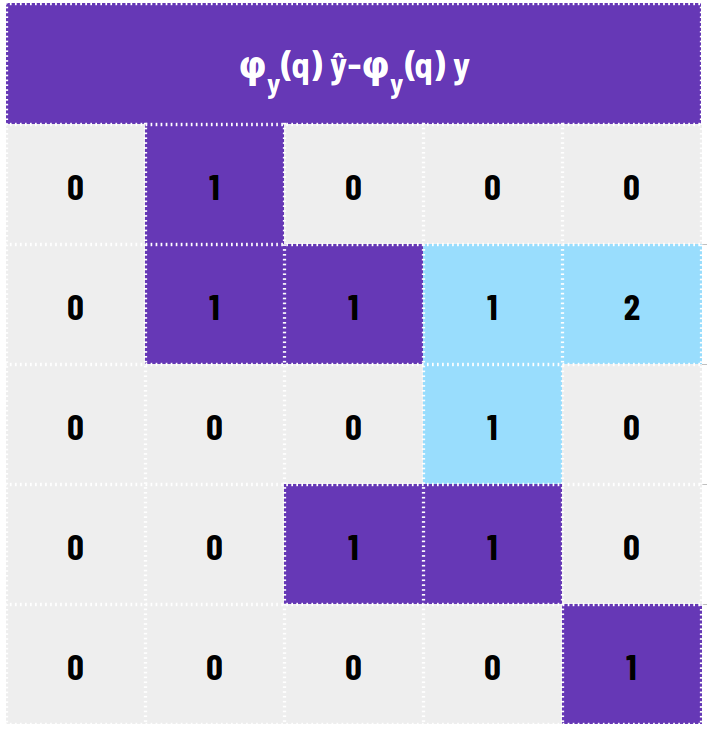
\includegraphics[width=\imgWidthFour]{images/boundary_final_4.png}}
    \caption[Final calculation of \ac{BL}]{Final calculation of \ac{BL} by precomputing the level set representation $\varphi_y(q)$ from the ground truth $y$ and multiplying it with the prediction $\hat{y}$ (b) and with the ground truth $y$ (c). To obtain the final boundary loss, the integrals $\int \varphi_y(q)\hat{y} dq$ and $\int \varphi_y(q)y dq$ are subtracted from each other (d).}
    \label{boundary_final}
\end{figure}

\subsection{Segmentation Metrics}
\label{subsec:segmentation_metrics}
Evaluating the performance of semantic segmentation models is critical to developing and optimizing practical algorithms for image understanding tasks. To assess the quality of a model's predictions, it is essential to utilize an appropriate measure to quantify the performance of the segmentation results. In this section, a variety of segmentation metrics commonly employed in classification tasks are explored. These metrics are the basis for comparing different models, understanding their strengths and weaknesses, and guiding further improvements. The following subsections will discuss each metric's underlying concepts, mathematical formulations, and practical applications, focusing on their relevance to semantic segmentation tasks.
\subsubsection*{Confusion Matrix}
\label{subsubsec:confusion_matrix}
Several of the following metrics use parts of the confusion matrix, a table used to describe the performance of a classification algorithm. The confusion matrix displays the number of correct and incorrect predictions made by the classifier. For semantic segmentation, the performance of each $\hat{y}\in \hat{Y}$ can be represented as a confusion matrix that summarizes all pixels within $\hat{y}$ as correct or incorrectly labeled. In the following, the rows of the confusion matrix represent the predicted class labels, while the columns represent the true (actual) class labels. The first cell in the first row represents the count of correctly classified as positive predictions.
In contrast, the second cell of the first row indicates the count of incorrectly classified as positive. The first cell in the second row represents the count of predictions incorrectly classified as negative, while the second cell correctly classified samples as negative. Even if confusion matrices exist for multi-class classification tasks, this work examines the binary case, which can be extended for multi-class classification. The confusion matrix for a binary classification problem has the following structure:
\begin{table}[H]
    \centering
    \begin{tabular}{c|c|c|}
        \cline{2-3}
                                                                                                                                           &
        \cellcolor[HTML]{000000}{\color[HTML]{FFFFFF} \begin{tabular}[c]{@{}c@{}}Actual \\ Positive\end{tabular}}                          &
        \cellcolor[HTML]{000000}{\color[HTML]{FFFFFF} \begin{tabular}[c]{@{}c@{}}Actual \\ Negative\end{tabular}}                            \\ \hline
        \multicolumn{1}{|c|}{\cellcolor[HTML]{000000}{\color[HTML]{FFFFFF} \begin{tabular}[c]{@{}c@{}}Predicted \\ Positive\end{tabular}}} &
        \cellcolor[HTML]{00A9CE}{\color[HTML]{FFFFFF} True Positive}                                                                       &
        \cellcolor[HTML]{99DDFD}{\color[HTML]{FFFFFF} False Positve}                                                                         \\ \hline
        \multicolumn{1}{|c|}{\cellcolor[HTML]{000000}{\color[HTML]{FFFFFF} \begin{tabular}[c]{@{}c@{}}Predicted \\ Negative\end{tabular}}} &
        \cellcolor[HTML]{6638B6}{\color[HTML]{FFFFFF} False Negative}                                                                      &
        \cellcolor[HTML]{9B7DD4}{\color[HTML]{FFFFFF} True Negative}                                                                         \\ \hline
    \end{tabular}
    \caption[Confusion matrix]{Structure of binary confusion matrix where the rows represent the predicted class labels while the cells represent the actual class. Each cell in the matrix represents the count of predictions where the true class is the column label, and the predicted class is the row label.}\label{tab:confusion_matrix}
\end{table}
Related to semantic segmentation, the values within the cells represent numbers of pixels described as follows:
\begin{itemize}[noitemsep]
    \item True Positive (TP): Number of correctly predicted pixels of the positive class
    \item False Positive (FP): Number of incorrectly predicted pixels of the positive class
    \item False Negative (FN): Number of incorrectly predicted pixels of the negative class
    \item True Negative (TN): Number of correctly predicted pixels of the negative class
\end{itemize}



\begin{figure}[H]%[htbp]
    \centering
    \subfigure[Output label]{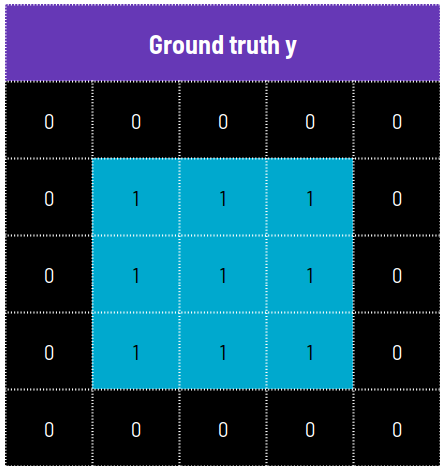
\includegraphics[width=\imgWidthTwo]{images/metrics_cm_gt.png}}
    \subfigure[Color coded prediction ]{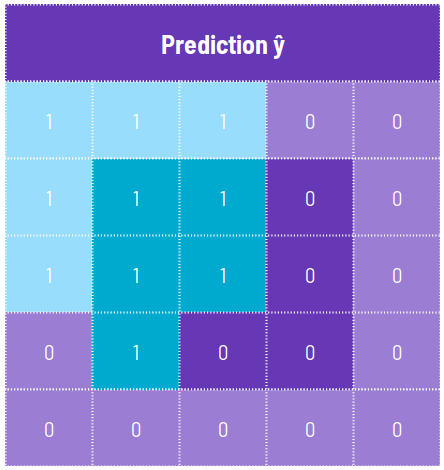
\includegraphics[width=\imgWidthTwo]{images/metrics_cm_yhat.png}}
    \caption[Output label and color-coded true/false positive/negative prediction]{Output label (a) and example of a 25-pixel visualization where each pixel is color-coded to indicate a \textbf{\textcolor{rwucyan}{True Positive}}, \textbf{\textcolor{rwucyanlight}{False Positive}}, \textbf{\textcolor{rwuviolet}{False Negative}} and \textbf{\textcolor{rwuvioletlight}{True Negative}} prediction (b) resulting in a confusion matrix of $\begin{bmatrix}5&5\\4&11\end{bmatrix}$.}
    \label{confusion_matrix_example}
\end{figure}
The following sections will describe some common metrics derived from the confusion matrix.

\subsubsection*{Precision (PPV), Recall (TPR)}
\label{subsubsec:precision_and_recall}
Precision and recall, also known as \ac{PPV} and \ac{TPR} are complementary metrics used to evaluate the performance of a classification task. The difference is that precision focuses on the number of false positives in addition to the true positives, while recall focuses on false negatives additionally to true positives.

The formal definition of precision and recall is as follows:
\begin{equation}
    \text{Precision}=\frac{TP}{TP+FP}
\end{equation}
\begin{equation}
    \text{Recall}=\frac{TP}{TP+FN}
\end{equation}
Intuitively, the perfect precision would have no false positives leading to a score of 1, while the perfect recall would have no false negatives, also leading to a score of 1. It is important to note that precision and recall are particularly relevant for the positive or foreground class in the context of semantic segmentation. \figref{precision_recall_metrics} illustrates two cases: one with high precision and low recall and the other with low precision and high recall. Based on the specific requirements and priorities of the segmentation task, a user might prefer one case over the other.

\begin{figure}[H]%[htbp]
    \centering
    \subfigure[High precision low recall]{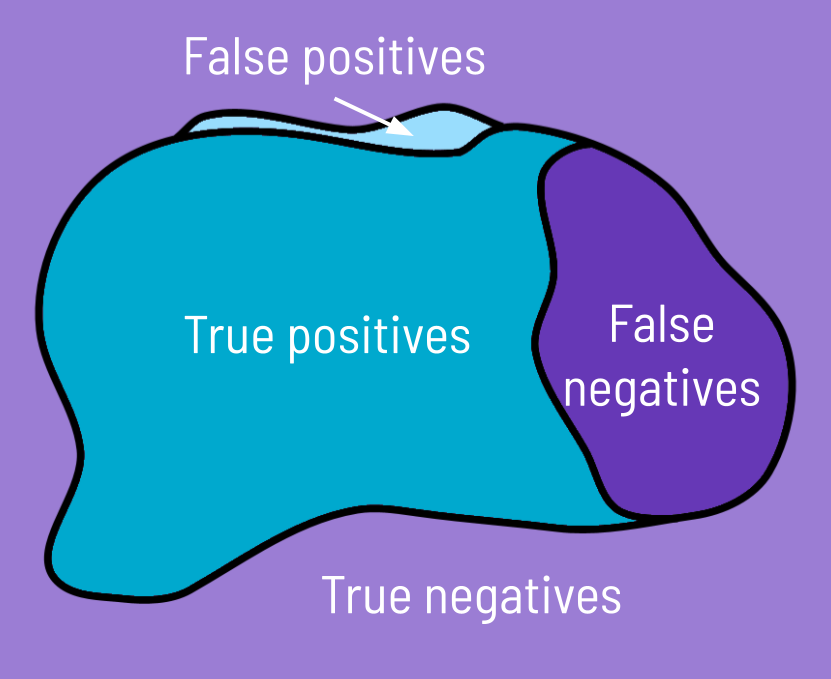
\includegraphics[width=\imgWidthTwo]{images/High_precision_low_recall_prototype.png}}
    \subfigure[Low precision high recall]{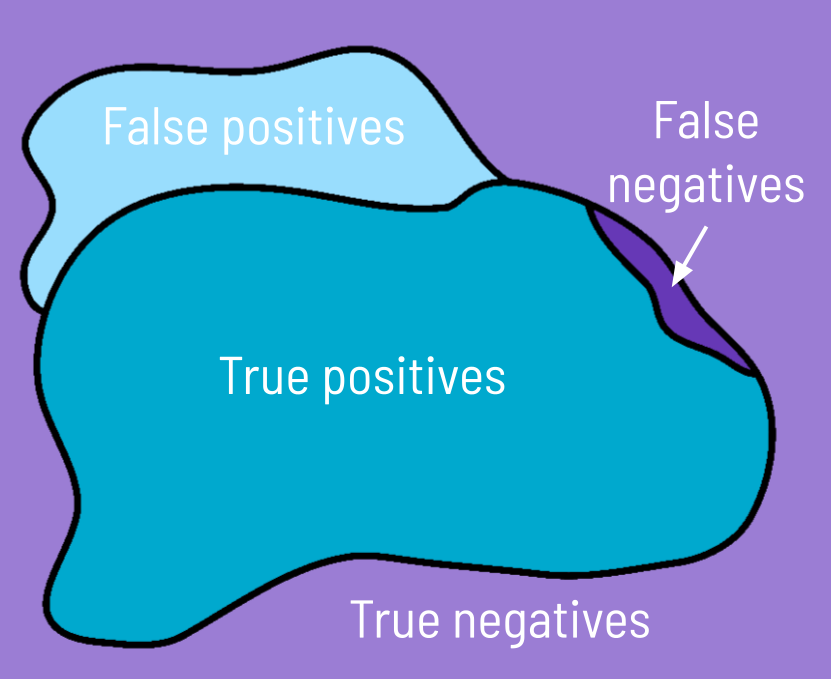
\includegraphics[width=\imgWidthTwo]{images/Low_precision_high_recall.png}}
    \caption[Precision and Recall]{Image (a) depicts a situation with very high precision. The false positives are very low. False negatives are high, which indicates a low recall. The situation in image (b) is the opposite, with a low precision and many false positives and a high recall with few false negatives.}
    \label{precision_recall_metrics}
\end{figure}

\subsubsection*{Specificity (TNR) and Negative Predictive Value (NPV)}
\label{subsubsec:specificity_and_negative_predictive_value}
Specificity, also known as \ac{TNR} and \ac{NPV}, are complementary metrics akin to precision and recall. However, these metrics emphasize true negatives instead of focusing on true positives. Specificity and \ac{NPV} are particularly useful in scenarios where the accurate identification of negative or background instances is crucial, such as in medical diagnostics \cite{Parikh2008-bd} or anomaly detection \cite{Henson2021}.

Specificity and negative predictive value are formally defined as follows:
\begin{equation}
    \text{Specificity}=\frac{TN}{TN+FP}
\end{equation}
\begin{equation}
    \text{Negative predictive value}=\frac{TN}{TN+FN}
\end{equation}
Intuitively, a perfect specificity score indicates no false positives, while a perfect \ac{NPV} implies no false negatives. In semantic segmentation, these metrics highlight the model's performance in correctly identifying negative or background classes.

\subsubsection*{Intersection over Union (IoU)}
\label{subsubsec:jaccard_index}
The \ac{IoU}, also known as the \ac{JI}, is a similarity measure used to compare two sample data objects. It is defined as the ratio of the intersection size to the union size \cite{Verma2020}.

Originally, the \ac{IoU} was described in set notation as:
\begin{equation}
    IOU=\frac{|A\cap B|}{|A \cup B|}=\frac{|A \cap B|}{|A|+|B|-|A\cap B|}
\end{equation}
where $A$ and $B$ represent two sets being compared.

In the context of confusion matrix components, the \ac{IoU} is defined as:
\begin{equation}
    IOU=\frac{TP}{TP+FP+FN}
\end{equation}
\subsubsection*{Dice Similarity Coefficient (DSC)}
\label{subsubsec:dice_similarity_coefficient}
The \ac{DSC}, also known as the \ac{SDI}, was originally defined in set notation to describe the similarity between two samples. It is a widely used measure for evaluating image segmentation algorithms, particularly within the medical field \cite{Carass2020-rj}. Given two sets, $A$ and $B$, the \ac{DSC} is defined as
\begin{equation}
    DSC=\frac{2|A\cap B|}{|A|+|B|}
\end{equation}
In terms of true positives (TP), false positives (FP), and false negatives (FN), the \ac{DSC} can be expressed as
\begin{equation}
    DSC=\frac{2\cdot TP}{2\cdot TP + FP + FN}
\end{equation}
Notably, true positives are counted twice in this measure, resulting in the \ac{DSC} having a higher value for the same number of correctly classified pixels than the \ac{IoU} metric.

\subsubsection*{Accuracy (Acc)}
\label{subsubsec:accuracy}
Accuracy measures the proportion of correctly classified pixels in an image defined as
\begin{equation}
    \text{Accuracy}=\frac{\text{Number of correctly classified pixels}}{\text{Total number of pixels}}
\end{equation}
where the number of correctly classified pixels also includes True Negative predictions. In terms of confusion matrix components, this metric can also be defined as
\begin{equation}
    \text{Accuracy}=\frac{TP+TN}{TP+TN+FP+FN}
\end{equation}

\subsubsection*{Multiclass Classification}
Previously, we discussed metric calculations for binary classification tasks involving only two classes. This concept can be extended to multi-class classification problems, where the output labels $y$ can be transformed from integers to one-hot-encoded format, as demonstrated in \figref{one_hot_encoded_mask}. With the predictions $\hat{y}$ provided in one-hot-encoded format, as shown in \figref{predictions_scores_softmax}, each class can be treated as a binary classification problem. To obtain a final metric score, we can calculate individual confusion matrices for each class and average the results. This approach is known as \texttt{macro averaging} and will be employed for this project. An alternative method, called \texttt{micro averaging}, involves calculating a single confusion matrix for all classes and using it to compute a single metric score. The following equations demonstrate the difference between these approaches for the \acf{IoU} metric.

\begin{equation}
    \text{Micro IoU} = \frac{\sum_{i=1}^{D} TP_i}{\sum_{i=1}^{D} (TP_i + FP_i + FN_i)}
    \label{eqn:micro_iou}
\end{equation}

\begin{equation}
    \text{Macro IoU} = \frac{1}{D} \sum_{i=1}^{D} \frac{TP_i}{(TP_i + FP_i + FN_i)}
    \label{eqn:macro_iou}
\end{equation}

Here, $D$ represents the number of classes, while $TP_i$, $FP_i$, and $FN_i$ denote the true positives, false positives, and false negatives for class $i$, respectively. \figref{multiclass_classification} further explores the differences between these approaches using an example that demonstrates metric calculation in an imbalanced situation.

\begin{figure}[H]
    \centering
    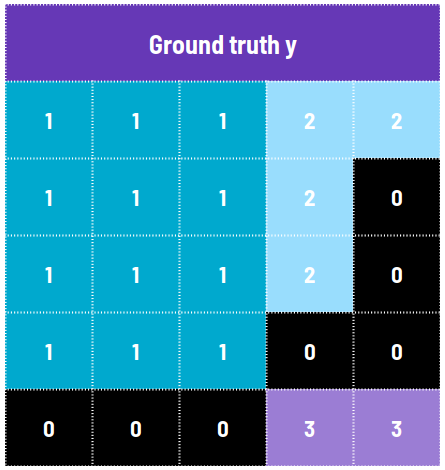
\includegraphics[width=\imgWidthTwo]{images/multiclass_example_y.png}
    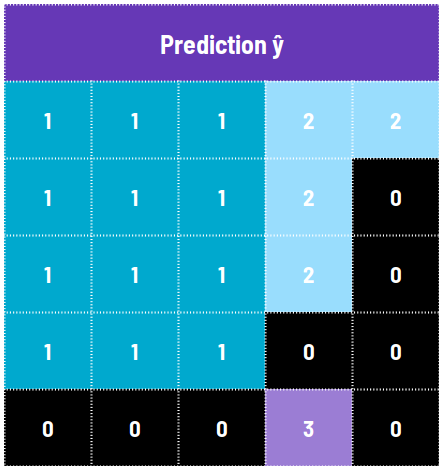
\includegraphics[width=\imgWidthTwo]{images/multiclass_example_yhat.png}
    \caption[Multiclass classification]{The \ac{IoU} using the micro average yields a value of $0.923$, whereas the macro \ac{IoU} average results in $0.843$. This significantly lower value for the 'macro' average primarily stems from the false negative prediction in pixel $\hat{Y}_{5,5}$, which leads to an \ac{IoU} score of $0.5$ for class three. According to equation \ref{eqn:macro_iou}, this prediction has a much larger impact on the overall result than in the micro \ac{IoU}, where the most prevalent class absorbs mispredictions for smaller classes. The prevalent class could be either the background or a foreground class with a considerably higher pixel count on average.}
    \label{multiclass_classification}
\end{figure}
\newpage

\subsection{Segmentation Architectures}
\label{subsec:segmentation_architectures}
The architecture employed in this project is derived from the U-Net, which is based on the \ac{EDA}. Introduced by \cite{DBLP:journals/corr/RonnebergerFB15} and illustrated in \figref{network_architecture}, the U-Net comprises two distinct paths: an encoding (contracting) path and a decoding (expanding) path, each composed of five layers. The encoding path incorporates pooling and convolutional operations along batch normalization and ReLU activation. It is responsible for capturing the context and reducing the spatial dimensions of the feature maps while increasing the number of channels. The decoding path upsamples the feature maps and concatenates them with the corresponding feature maps from the encoding path to provide high-resolution spatial information. After concatenation, the convolutions are applied to refine the feature maps. In this example, the final layer is a 1x1 convolution that maps the feature maps to the desired number of output classes resulting in a binary segmentation mask of shape 2x256x256 where each channel corresponds to one of the two classes in the binary segmentation.\cite{DBLP:journals/corr/RonnebergerFB15}
\begin{figure}[H]%[htbp]
    \centering
    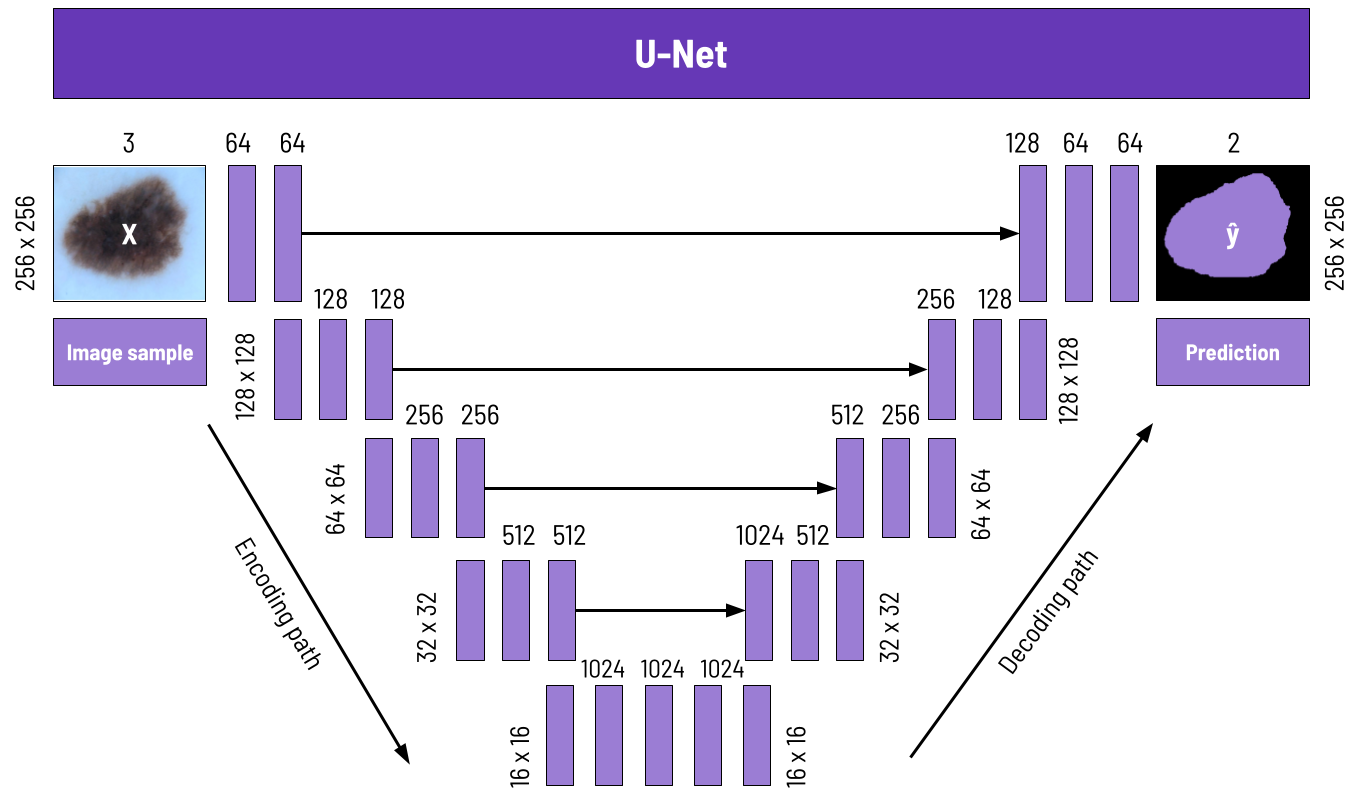
\includegraphics[width=\imgWidthXL]{images/NetworkArchitecture.png}
    \caption[U-Net]{U-Net model architecture proposed by \cite{DBLP:journals/corr/RonnebergerFB15}}
    \label{network_architecture}
\end{figure}
Besides the U-Net architecture, there is a wide variety of further models. \cite{doi:10.1080/08839514.2022.2032924} provides an excellent survey on deep learning architectures for semantic segmentation such as the \ac{SPP} \cite{doi:10.1080/08839514.2022.2032924} or the DeepLabv3+ Architecture\cite{Chen_2018_ECCV}.

\subsection{Segmentation Framework}
\label{subsec:segmentation_framework}
A segmentation framework follows a similar implementation as a standard deep learning framework presented as a model production cycle in \figref{model_production_cycle}, which entails configuration, preprocessing, training, validation, testing, and monitoring.
\begin{figure}[H]%[htbp]
    \centering
    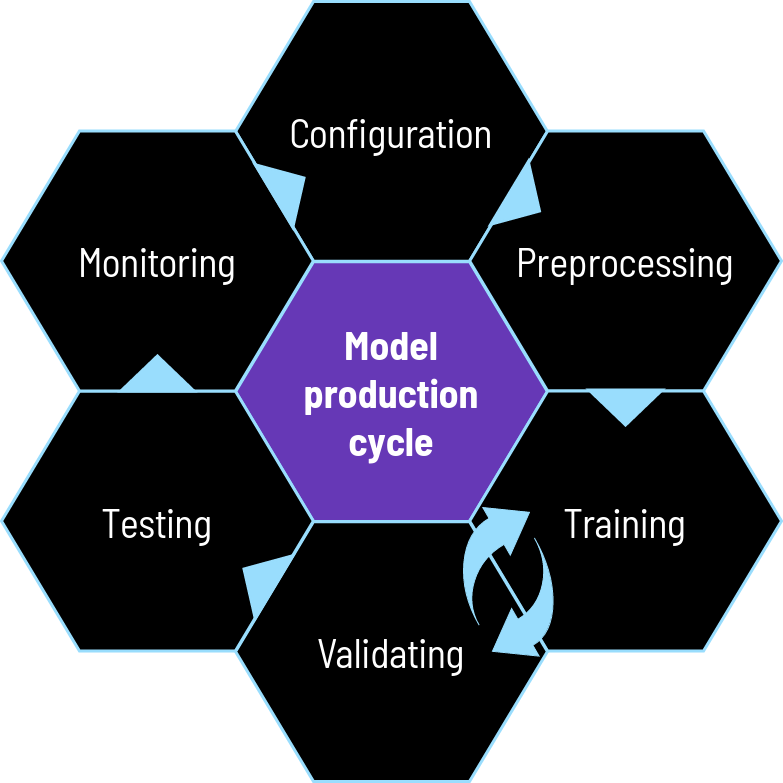
\includegraphics[width=\imgWidthM]{images/model_production_cycle.png}
    \caption[Experimental setup]{The model production cycle iteratively preprocesses, trains, validates, tests, and logs the results of each model using a specified configuration.}
    \label{model_production_cycle}
\end{figure}

\begin{enumerate}
    \item \textbf{\emph{Configuration}}: The configuration generally entails setting up the parameters used to train the model. There are various ways to efficiently search for hyperparameters, with the selection ultimately depending on several factors such as dataset size, computational resources, and chosen network architecture.
    \item \textbf{\emph{Preprocessing}}: The preprocessing step involves preparing the data for input into the model, which includes tasks such as data augmentation, normalization, and encoding of categorical features. This step ensures that the data is in a suitable training, validation, and testing format.
    \item \textbf{\emph{Training}}: The training process begins by iterating through all samples in the training set. For each input sample $x$, the model generates a prediction $\hat{y}$ and calculates a loss $l(\hat{y},y)$, which is used to adjust the models' weights via backpropagation which typically involves the optimization technique called gradient descent as discussed earlier. An optimizer such as the Adam optimizer can effectively determine an appropriate learning rate, also called step size for gradient descent, as it utilizes an adaptive learning rate for each parameter during the backpropagation process. Once this process is done for every sample, label pair within the training set, the model will be validated in the next step.
    \item \textbf{\emph{Validation}}: After completing the training steps, the validation step is carried out to assess the trained models' performance by generating predictions and testing them against the corresponding output labels from the validation set. No model parameter updates occur during this step. Once the validation steps are finished, the process begins anew with the training set. This cycle repeats until all epochs have been completed. Epochs refer to a single pass through the entire training dataset while training a model.
    \item \textbf{\emph{Testing}}: Finally, the testing step is performed on the test data, which has been previously separated from the entire dataset. The test data results are crucial for evaluating a model's performance, as they reveal its generalization capabilities on unseen data. Like the validation step, the model parameters remain unchanged during the test step.
    \item \textbf{\emph{Monitoring}}: Monitoring is a crucial part of the model production cycle as it helps track the progress of the training, validation, and testing processes, allowing for the detection of potential issues or improvements. This step includes logging performance metrics, visualizing model performance, and saving intermediate results for later analysis.
\end{enumerate}
